% Options for packages loaded elsewhere
\PassOptionsToPackage{unicode}{hyperref}
\PassOptionsToPackage{hyphens}{url}
%
\documentclass[
]{article}
\usepackage{amsmath,amssymb}
\usepackage{iftex}
\ifPDFTeX
  \usepackage[T1]{fontenc}
  \usepackage[utf8]{inputenc}
  \usepackage{textcomp} % provide euro and other symbols
\else % if luatex or xetex
  \usepackage{unicode-math} % this also loads fontspec
  \defaultfontfeatures{Scale=MatchLowercase}
  \defaultfontfeatures[\rmfamily]{Ligatures=TeX,Scale=1}
\fi
\usepackage{lmodern}
\ifPDFTeX\else
  % xetex/luatex font selection
\fi
% Use upquote if available, for straight quotes in verbatim environments
\IfFileExists{upquote.sty}{\usepackage{upquote}}{}
\IfFileExists{microtype.sty}{% use microtype if available
  \usepackage[]{microtype}
  \UseMicrotypeSet[protrusion]{basicmath} % disable protrusion for tt fonts
}{}
\makeatletter
\@ifundefined{KOMAClassName}{% if non-KOMA class
  \IfFileExists{parskip.sty}{%
    \usepackage{parskip}
  }{% else
    \setlength{\parindent}{0pt}
    \setlength{\parskip}{6pt plus 2pt minus 1pt}}
}{% if KOMA class
  \KOMAoptions{parskip=half}}
\makeatother
\usepackage{xcolor}
\usepackage[margin=1in]{geometry}
\usepackage{color}
\usepackage{fancyvrb}
\newcommand{\VerbBar}{|}
\newcommand{\VERB}{\Verb[commandchars=\\\{\}]}
\DefineVerbatimEnvironment{Highlighting}{Verbatim}{commandchars=\\\{\}}
% Add ',fontsize=\small' for more characters per line
\usepackage{framed}
\definecolor{shadecolor}{RGB}{248,248,248}
\newenvironment{Shaded}{\begin{snugshade}}{\end{snugshade}}
\newcommand{\AlertTok}[1]{\textcolor[rgb]{0.94,0.16,0.16}{#1}}
\newcommand{\AnnotationTok}[1]{\textcolor[rgb]{0.56,0.35,0.01}{\textbf{\textit{#1}}}}
\newcommand{\AttributeTok}[1]{\textcolor[rgb]{0.13,0.29,0.53}{#1}}
\newcommand{\BaseNTok}[1]{\textcolor[rgb]{0.00,0.00,0.81}{#1}}
\newcommand{\BuiltInTok}[1]{#1}
\newcommand{\CharTok}[1]{\textcolor[rgb]{0.31,0.60,0.02}{#1}}
\newcommand{\CommentTok}[1]{\textcolor[rgb]{0.56,0.35,0.01}{\textit{#1}}}
\newcommand{\CommentVarTok}[1]{\textcolor[rgb]{0.56,0.35,0.01}{\textbf{\textit{#1}}}}
\newcommand{\ConstantTok}[1]{\textcolor[rgb]{0.56,0.35,0.01}{#1}}
\newcommand{\ControlFlowTok}[1]{\textcolor[rgb]{0.13,0.29,0.53}{\textbf{#1}}}
\newcommand{\DataTypeTok}[1]{\textcolor[rgb]{0.13,0.29,0.53}{#1}}
\newcommand{\DecValTok}[1]{\textcolor[rgb]{0.00,0.00,0.81}{#1}}
\newcommand{\DocumentationTok}[1]{\textcolor[rgb]{0.56,0.35,0.01}{\textbf{\textit{#1}}}}
\newcommand{\ErrorTok}[1]{\textcolor[rgb]{0.64,0.00,0.00}{\textbf{#1}}}
\newcommand{\ExtensionTok}[1]{#1}
\newcommand{\FloatTok}[1]{\textcolor[rgb]{0.00,0.00,0.81}{#1}}
\newcommand{\FunctionTok}[1]{\textcolor[rgb]{0.13,0.29,0.53}{\textbf{#1}}}
\newcommand{\ImportTok}[1]{#1}
\newcommand{\InformationTok}[1]{\textcolor[rgb]{0.56,0.35,0.01}{\textbf{\textit{#1}}}}
\newcommand{\KeywordTok}[1]{\textcolor[rgb]{0.13,0.29,0.53}{\textbf{#1}}}
\newcommand{\NormalTok}[1]{#1}
\newcommand{\OperatorTok}[1]{\textcolor[rgb]{0.81,0.36,0.00}{\textbf{#1}}}
\newcommand{\OtherTok}[1]{\textcolor[rgb]{0.56,0.35,0.01}{#1}}
\newcommand{\PreprocessorTok}[1]{\textcolor[rgb]{0.56,0.35,0.01}{\textit{#1}}}
\newcommand{\RegionMarkerTok}[1]{#1}
\newcommand{\SpecialCharTok}[1]{\textcolor[rgb]{0.81,0.36,0.00}{\textbf{#1}}}
\newcommand{\SpecialStringTok}[1]{\textcolor[rgb]{0.31,0.60,0.02}{#1}}
\newcommand{\StringTok}[1]{\textcolor[rgb]{0.31,0.60,0.02}{#1}}
\newcommand{\VariableTok}[1]{\textcolor[rgb]{0.00,0.00,0.00}{#1}}
\newcommand{\VerbatimStringTok}[1]{\textcolor[rgb]{0.31,0.60,0.02}{#1}}
\newcommand{\WarningTok}[1]{\textcolor[rgb]{0.56,0.35,0.01}{\textbf{\textit{#1}}}}
\usepackage{graphicx}
\makeatletter
\def\maxwidth{\ifdim\Gin@nat@width>\linewidth\linewidth\else\Gin@nat@width\fi}
\def\maxheight{\ifdim\Gin@nat@height>\textheight\textheight\else\Gin@nat@height\fi}
\makeatother
% Scale images if necessary, so that they will not overflow the page
% margins by default, and it is still possible to overwrite the defaults
% using explicit options in \includegraphics[width, height, ...]{}
\setkeys{Gin}{width=\maxwidth,height=\maxheight,keepaspectratio}
% Set default figure placement to htbp
\makeatletter
\def\fps@figure{htbp}
\makeatother
\setlength{\emergencystretch}{3em} % prevent overfull lines
\providecommand{\tightlist}{%
  \setlength{\itemsep}{0pt}\setlength{\parskip}{0pt}}
\setcounter{secnumdepth}{5}
\ifLuaTeX
  \usepackage{selnolig}  % disable illegal ligatures
\fi
\usepackage{bookmark}
\IfFileExists{xurl.sty}{\usepackage{xurl}}{} % add URL line breaks if available
\urlstyle{same}
\hypersetup{
  pdftitle={Binned Analysis},
  pdfauthor={Emanuele Coradin and Dario Puggioni},
  hidelinks,
  pdfcreator={LaTeX via pandoc}}

\title{Binned Analysis}
\author{Emanuele Coradin and Dario Puggioni}
\date{2024-06-25}

\begin{document}
\maketitle

{
\setcounter{tocdepth}{2}
\tableofcontents
}
\section{\texorpdfstring{Bayesian analysis of the \(\mu\) lifetime and
g-2 parameter with \(\mu\)
SR}{Bayesian analysis of the \textbackslash mu lifetime and g-2 parameter with \textbackslash mu SR}}\label{bayesian-analysis-of-the-mu-lifetime-and-g-2-parameter-with-mu-sr}

\subsection{Introduction}\label{introduction}

Muons are long-lived particles, produced in the decays of pions and
kaons originating from the interactions of primary cosmic rays with the
Earth's atmosphere.

Moreover, parity violation is also present in the decay which proceeds
as follow: \(\mu^+ \rightarrow e^+ + \nu_e + \overline{\nu_\mu}\) and
\(\mu^- \rightarrow e^- + \overline{\nu_e} + \nu_\mu\).

Simple experiments can be performed by measuring muons that decay in a
thick absorber. If the absorber is immersed in a constant magnetic
field, the muon spin, before the decay, precesses with its Larmor
frequency \(\omega_L = g_{\mu} \frac{eB}{2 m_{\mu} c}\).

The decay proceeds mainly along the direction of the spin of the muon
and therefore, if the muon is (partly) polarized, the detected signal
varies with time with \(\omega_L\). Analyzing the data collected without
and with the magnetic field, we set up a Markov Chain Monte Carlo that
allows us to extract the muon lifetime \(\tau\), with the magnetic field
turned off, and the muon precession frequency with the magnetic field
turned on.

In this document we are presenting a conventional kind of analysis, by
building an histogram and then fitting it with a curve. The value of the
parameters are inferred in a Bayesian framework.

\subsection{Description of the data
analysis}\label{description-of-the-data-analysis}

We have at our disposal two datasets: `Lifetime' and `Precession'. The
former contains the measurements of the time difference between the muon
(antimuon) and electron (positron) signals with the magnetic field
turned off, while in the latter the measurements are taken with a
magnetic field \(B=5.6\ \text{mT}\). To convert the ADC counts in
seconds we use the results of a previous calibration measurement: \$ t =
p\_0 + \text{ADC} \cdot p\_1 \$, where
\(p_0 = (7.4 \pm 4.4)\ \text{ns}\) and \$ p\_1 = (14.90
\pm 0.11)~\text{ns} \$.

In particular, since the electron could also undergo nuclear capture,
the vast majority of the signals are made of positrons.

Defining N(t) as the number of observed decays at time t + dt, we expect
it to follow the rule \$ N(t) = N\_0 e\^{}\{- \frac{t}{\tau}\} + c \$ in
the Lifetime dataset, with c modeling a constant background.

If the magnetic field is turned on, we expect instead a different law
due to the precession of the antimuon: \$N(t) = N\_0 e\^{}\{-\frac {t}
\{\tau\}\} \cdot (1+\alpha \cos(\omega\_L t + \delta))+ c \(.\)\alpha\$
is an asymmetry parameter originating from the parity violation.

The analytic form of the differential emission probability per unit of
time of the positron is in fact: \[
d\Gamma = W(\varepsilon, \theta) \, d\varepsilon \, d\Omega = \frac{1}{4\pi \tau} \cdot 2\varepsilon^2 (3 - 2\varepsilon) \left[ 1 + \frac{2\varepsilon - 1}{3 - 2\varepsilon} \cos \theta \right] d\varepsilon \, d\Omega = \frac{1}{4\pi \tau} \cdot K(\varepsilon)[1+a(\varepsilon) \cos(\theta)] d\varepsilon \, d\Omega
\],

where \(\epsilon = \frac{\text{E}}{\text{E}_{\text{max}}}\),
\(K(\varepsilon) = 2\varepsilon^2(3-2\varepsilon)\),
\(a(\varepsilon) = \frac{2\varepsilon-1}{3-2\varepsilon}\),
\(\text{E}_{\text{max}} \approx 53.83\ \text{MeV}\), \(\theta=0\) is the
spin direction.

The asymmetry term is thus
\(\alpha(\varepsilon) = K(\varepsilon)a(\varepsilon)\), and it's energy
dependent with support \(\alpha\in \left[ -\frac 1 3,\ 1 \right]\). We
can calculate its mean value and variance: -
\(\bar{\alpha} = \int_0^1 \alpha(\varepsilon) \, d\varepsilon= \frac{1}{3}\)
-
\(\text{Var}[\alpha] = \int_0^1 (\alpha(\varepsilon)-\bar{\alpha})^2 \, d\varepsilon \approx 0.3\)

This derivation is valid in the hypothesis of maximum and equal
detection efficiency for every energy in the spectrum. In practice,
however, its mean value is considerably lower.

Furthermore, the angular distribution of cosmic muons is experimentally
close to \(P(\theta) = I_0 \cos^2(\theta)\), where \(\theta\) is the
azimuthal angle.

Considering a detector characterized by a cylindrical symmetry along the
azimuth direction, and immersed in a uniform transverse magnetic field
\(B\), we can extrapolate that the pdf of observing a decay at time
\(t\) is \[
P(t) = \frac{e^{-\frac{t}{\tau}} (1+\alpha \cos(\omega_L t + \delta))}{Z}
\] with \(\alpha\) accounting for the experimental asymmetry, and
\(\delta\) modeling errors in the definition of the time zero or angular
misalignments.

\subsection{Choice of the priors}\label{choice-of-the-priors}

\subsubsection{\texorpdfstring{Muon Lifetime
\(\tau\)}{Muon Lifetime \textbackslash tau}}\label{muon-lifetime-tau}

For the muon lifetime \(\tau\), we assume a prior that reflects our
prior knowledge based on similar previous experiments:

\begin{itemize}
\tightlist
\item
  Amsler: \(\tau = (2.10\pm0.05)\ \mu\text{s}\);
\item
  Bosnam: \(\tau = (2.16\pm0.02)\ \mu\text{s}\) and
  \(\tau = (2.07\pm0.02)\ \mu\text{s}\)
\end{itemize}

Considering a weighted average of them, we obtain a prior mean of
\(\bar{\tau_{\text{prior}}} = 2.11\  \mu\text{s}\) with standard
deviation of \(\text{SD}[{\tau_{\text{prior}}}] = 0.01  \mu\text{s}\)

Therefore, we decide to model the prior with a gamma distribution of
parameters \(\alpha\) and \(\beta\) tuned to satisfy these conditions.

\subsubsection{\texorpdfstring{Asimmetry parameter
\(\alpha\)}{Asimmetry parameter \textbackslash alpha}}\label{asimmetry-parameter-alpha}

The most conservative choice would be a prior fully based on the
theoretical aspects mentioned above. Nevertheless, since the
experimental setup is similar to the one used in the previous
experiments we previously cited, we decide again to use them:

\begin{itemize}
\tightlist
\item
  Amsler: \(\alpha = 0.067 \pm 0.011\);
\item
  Bosnam: \(\alpha = 0.05  \pm 0.01\) and \(\alpha = 0.06  \pm 0.01\).
\end{itemize}

This time we are more conservative, choosing a prior mean of 0.06 with a
standard deviation of 0.01. We model the pdf using a re scaled and
shifted Beta distribution, having support in
\(\alpha\in \left[-\frac 1 3,\ 1 \right]\).

\subsubsection{\texorpdfstring{Larmor frequency
\(\omega_L\)}{Larmor frequency \textbackslash omega\_L}}\label{larmor-frequency-omega_l}

Recall that the Larmor frequency formula is
\(\omega_L = g_{\mu} \frac {eB} {2 m_{\mu} c}\). Considering
\(g_{\mu}=2\), the magnetic field \(B=5.6\ \text{mT} \pm 2\%\), and all
the other known constants, we can calculate the expected value to be
\(\omega_L = 4.77\ \text{MHz}\).

The main source of error in this estimate is by far the uncertainty in
the magnetic field. Assuming a uniform distribution, we can convert the
maximum error in a casual one
\(\sigma_B = \frac {\Delta B} {\sqrt{12}}\). Projecting this back to the
Larmor frequency, we can estimate its casual error to be
\(\sigma_{\omega_L} = 0.06\ \text{mT}\).

Therefore, we decide to model the prior with a gamma distribution of
parameters \(\alpha\) and \(\beta\) tuned to satisfy these conditions.

\subsubsection{\texorpdfstring{Initial phase
\(\delta\)}{Initial phase \textbackslash delta}}\label{initial-phase-delta}

Given the theoretical considerations made above, considering the
experimental evidence that the probability of observing a cosmic muon at
the azimuthal angle \(\theta\) is \(P(\theta) = I_0 \cos^2(\theta)\), we
expect the mean value to be 0 with a variance
\(\text{Var}[\theta]= \int_{-\frac \pi 2}^{\frac \pi 2} I_0 \theta^2 \cos^2(\theta)\ d\theta = 0.32\).

Again, we model the prior distribution with a rescaled and shifted beta
distribution, in order to have support in
\(\theta \in \left [-\frac \pi 2, \frac \pi 2 \right]\) and those
moments.

\subsubsection{\texorpdfstring{\(N_0\) and
c}{N\_0 and c}}\label{n_0-and-c}

These parameters are modeling the number of true observed decays and the
background rate. Since they depend both on the time of measurement and
the behaviour of the all detector they are really difficult to estimate,
so we decide to take just a uniform prior.

\subsection{Functions and default
values}\label{functions-and-default-values}

\begin{Shaded}
\begin{Highlighting}[]
\CommentTok{\# {-}{-}{-}{-}{-}{-}{-} Analytical calculations {-}{-}{-}{-}{-}{-}{-}{-}{-}{-}{-}}

\NormalTok{getGammaParam }\OtherTok{\textless{}{-}} \ControlFlowTok{function}\NormalTok{(mean, variance) \{}
\NormalTok{  beta }\OtherTok{\textless{}{-}}\NormalTok{ mean }\SpecialCharTok{/}\NormalTok{ variance}
\NormalTok{  alpha }\OtherTok{\textless{}{-}}\NormalTok{ mean }\SpecialCharTok{*}\NormalTok{ beta}
  \FunctionTok{c}\NormalTok{(}\AttributeTok{alpha =}\NormalTok{ alpha, }\AttributeTok{beta =}\NormalTok{ beta)}
\NormalTok{\}}

\NormalTok{getBetaParam }\OtherTok{\textless{}{-}} \ControlFlowTok{function}\NormalTok{(mean, variance) \{}
\NormalTok{  nu }\OtherTok{\textless{}{-}}\NormalTok{ mean }\SpecialCharTok{*}\NormalTok{ (mean }\SpecialCharTok{*}\NormalTok{ (}\DecValTok{1} \SpecialCharTok{{-}}\NormalTok{ mean) }\SpecialCharTok{/}\NormalTok{ variance }\SpecialCharTok{{-}} \DecValTok{1}\NormalTok{)}
\NormalTok{  alpha }\OtherTok{\textless{}{-}}\NormalTok{ mean }\SpecialCharTok{*}\NormalTok{ nu}
\NormalTok{  beta }\OtherTok{\textless{}{-}}\NormalTok{ nu }\SpecialCharTok{*}\NormalTok{ (}\DecValTok{1} \SpecialCharTok{{-}}\NormalTok{ mean)}
  \FunctionTok{c}\NormalTok{(}\AttributeTok{alpha =}\NormalTok{ alpha, }\AttributeTok{beta =}\NormalTok{ beta)}
\NormalTok{\}}

\CommentTok{\# {-}{-}{-}{-}{-}{-}{-}{-} Functions for plotting {-}{-}{-}{-}{-}{-}{-}{-}{-}{-}{-}}

\NormalTok{plotdata }\OtherTok{\textless{}{-}} \ControlFlowTok{function}\NormalTok{(data, }\AttributeTok{title =} \ConstantTok{NULL}\NormalTok{, }\AttributeTok{xlab =} \FunctionTok{expression}\NormalTok{(Delta }\SpecialCharTok{*}\NormalTok{ T }\SpecialCharTok{\textasciitilde{}} \StringTok{"["} \SpecialCharTok{*}\NormalTok{ mu }\SpecialCharTok{*} \StringTok{"s"} \SpecialCharTok{*} \StringTok{"]"}\NormalTok{), }\AttributeTok{histdata =} \ConstantTok{NULL}\NormalTok{, }\AttributeTok{scale =} \StringTok{\textquotesingle{}lin\textquotesingle{}}\NormalTok{, }\AttributeTok{bins =}\NormalTok{ bins\_default, }\AttributeTok{plot\_histbar =} \ConstantTok{FALSE}\NormalTok{, }\AttributeTok{xlim =} \ConstantTok{NULL}\NormalTok{, }\AttributeTok{ylim=}\ConstantTok{NULL}\NormalTok{) \{}
  \ControlFlowTok{if}\NormalTok{ (}\FunctionTok{is.null}\NormalTok{(histdata)) histdata }\OtherTok{\textless{}{-}} \FunctionTok{hist}\NormalTok{(data, }\AttributeTok{breaks =}\NormalTok{ bins, }\AttributeTok{plot =} \ConstantTok{FALSE}\NormalTok{)}

\NormalTok{  df }\OtherTok{\textless{}{-}} \FunctionTok{data.frame}\NormalTok{(}\AttributeTok{mids =}\NormalTok{ histdata}\SpecialCharTok{$}\NormalTok{mids, }\AttributeTok{counts =}\NormalTok{ histdata}\SpecialCharTok{$}\NormalTok{counts)}

  \ControlFlowTok{if}\NormalTok{ (scale }\SpecialCharTok{==} \StringTok{"lin"}\NormalTok{) \{}
\NormalTok{    df }\OtherTok{\textless{}{-}}\NormalTok{ df }\SpecialCharTok{\%\textgreater{}\%} \FunctionTok{mutate}\NormalTok{(}\AttributeTok{se =} \FunctionTok{sqrt}\NormalTok{(counts))  }\CommentTok{\# Errore standard come sqrt dei counts (assunzione di distribuzione di Poisson)}
\NormalTok{  \} }\ControlFlowTok{else}\NormalTok{ \{}
\NormalTok{    df }\OtherTok{\textless{}{-}}\NormalTok{ df }\SpecialCharTok{\%\textgreater{}\%} \FunctionTok{mutate}\NormalTok{(}\AttributeTok{se =} \DecValTok{1} \SpecialCharTok{/}\NormalTok{ (}\FunctionTok{log}\NormalTok{(}\DecValTok{10}\NormalTok{)}\SpecialCharTok{*}\FunctionTok{sqrt}\NormalTok{(counts)))  }\CommentTok{\# Errore standard come 1/sqrt(counts)}
\NormalTok{  \}}

\NormalTok{  p }\OtherTok{\textless{}{-}} \FunctionTok{ggplot}\NormalTok{() }\SpecialCharTok{+}
    \FunctionTok{theme\_minimal}\NormalTok{() }\SpecialCharTok{+}
    \FunctionTok{ggtitle}\NormalTok{(title) }\SpecialCharTok{+}
    \FunctionTok{labs}\NormalTok{(}\AttributeTok{x =}\NormalTok{ xlab, }\AttributeTok{y =} \FunctionTok{ifelse}\NormalTok{(scale }\SpecialCharTok{==} \StringTok{"lin"}\NormalTok{, }\StringTok{"Counts"}\NormalTok{, }\FunctionTok{expression}\NormalTok{(log[}\DecValTok{10}\NormalTok{](Counts))), }\AttributeTok{color =} \StringTok{"Legend"}\NormalTok{) }\SpecialCharTok{+}
    \FunctionTok{theme}\NormalTok{(}\AttributeTok{plot.title =} \FunctionTok{element\_text}\NormalTok{(}\AttributeTok{face =} \StringTok{"bold"}\NormalTok{, }\AttributeTok{size =} \DecValTok{14}\NormalTok{),}
          \AttributeTok{axis.title.x =} \FunctionTok{element\_text}\NormalTok{(}\AttributeTok{size =} \DecValTok{12}\NormalTok{),}
          \AttributeTok{axis.title.y =} \FunctionTok{element\_text}\NormalTok{(}\AttributeTok{size =} \DecValTok{12}\NormalTok{))}

  \ControlFlowTok{if}\NormalTok{ (plot\_histbar) \{}
\NormalTok{    p }\OtherTok{\textless{}{-}}\NormalTok{ p }\SpecialCharTok{+} \FunctionTok{geom\_bar}\NormalTok{(}\AttributeTok{data =}\NormalTok{ df, }\FunctionTok{aes}\NormalTok{(}\AttributeTok{x =}\NormalTok{ mids, }\AttributeTok{y =}\NormalTok{ counts), }\AttributeTok{fill =} \StringTok{\textquotesingle{}blue\textquotesingle{}}\NormalTok{, }\AttributeTok{color =} \StringTok{\textquotesingle{}blue\textquotesingle{}}\NormalTok{)}
    \ControlFlowTok{if}\NormalTok{ (scale }\SpecialCharTok{==} \StringTok{"log"}\NormalTok{) \{}
\NormalTok{      p }\OtherTok{\textless{}{-}}\NormalTok{ p }\SpecialCharTok{+} \FunctionTok{scale\_y\_log10}\NormalTok{()}
\NormalTok{    \}}
\NormalTok{  \} }\ControlFlowTok{else}\NormalTok{ \{}
    \ControlFlowTok{if}\NormalTok{ (scale }\SpecialCharTok{==} \StringTok{"lin"}\NormalTok{) \{}
\NormalTok{      p }\OtherTok{\textless{}{-}}\NormalTok{ p }\SpecialCharTok{+}
        \FunctionTok{geom\_point}\NormalTok{(}\AttributeTok{data =}\NormalTok{ df, }\FunctionTok{aes}\NormalTok{(}\AttributeTok{x =}\NormalTok{ mids, }\AttributeTok{y =}\NormalTok{ counts), }\AttributeTok{color =} \StringTok{\textquotesingle{}blue\textquotesingle{}}\NormalTok{, }\AttributeTok{size =} \DecValTok{1}\NormalTok{) }\SpecialCharTok{+}
        \FunctionTok{geom\_errorbar}\NormalTok{(}\AttributeTok{data =}\NormalTok{ df, }\FunctionTok{aes}\NormalTok{(}\AttributeTok{x =}\NormalTok{ mids, }\AttributeTok{ymin =}\NormalTok{ counts }\SpecialCharTok{{-}}\NormalTok{ se, }\AttributeTok{ymax =}\NormalTok{ counts }\SpecialCharTok{+}\NormalTok{ se), }\AttributeTok{color =} \StringTok{\textquotesingle{}red\textquotesingle{}}\NormalTok{, }\AttributeTok{width =} \FloatTok{0.2}\NormalTok{, }\AttributeTok{size =} \FloatTok{0.5}\NormalTok{, }\AttributeTok{alpha =} \FloatTok{0.6}\NormalTok{)}
\NormalTok{    \} }\ControlFlowTok{else}\NormalTok{ \{}
\NormalTok{      p }\OtherTok{\textless{}{-}}\NormalTok{ p }\SpecialCharTok{+}
        \FunctionTok{geom\_point}\NormalTok{(}\AttributeTok{data =}\NormalTok{ df, }\FunctionTok{aes}\NormalTok{(}\AttributeTok{x =}\NormalTok{ mids, }\AttributeTok{y =} \FunctionTok{log10}\NormalTok{(counts)), }\AttributeTok{color =} \StringTok{\textquotesingle{}blue\textquotesingle{}}\NormalTok{, }\AttributeTok{size =} \DecValTok{1}\NormalTok{) }\SpecialCharTok{+}
        \FunctionTok{geom\_errorbar}\NormalTok{(}\AttributeTok{data =}\NormalTok{ df, }\FunctionTok{aes}\NormalTok{(}\AttributeTok{x =}\NormalTok{ mids, }\AttributeTok{ymin =} \FunctionTok{log10}\NormalTok{(counts) }\SpecialCharTok{{-}}\NormalTok{ se, }\AttributeTok{ymax =} \FunctionTok{log10}\NormalTok{(counts) }\SpecialCharTok{+}\NormalTok{ se), }\AttributeTok{color =} \StringTok{\textquotesingle{}red\textquotesingle{}}\NormalTok{, }\AttributeTok{width =} \FloatTok{0.2}\NormalTok{, }\AttributeTok{size =} \FloatTok{0.5}\NormalTok{, }\AttributeTok{alpha =} \FloatTok{0.6}\NormalTok{)}
\NormalTok{    \}}
\NormalTok{  \}}

  \ControlFlowTok{if}\NormalTok{ (}\SpecialCharTok{!}\FunctionTok{is.null}\NormalTok{(xlim)) \{}
\NormalTok{    p }\OtherTok{\textless{}{-}}\NormalTok{ p }\SpecialCharTok{+} \FunctionTok{xlim}\NormalTok{(xlim)}
\NormalTok{  \}}
  \ControlFlowTok{if}\NormalTok{ (}\SpecialCharTok{!}\FunctionTok{is.null}\NormalTok{(ylim)) \{}
\NormalTok{    p }\OtherTok{\textless{}{-}}\NormalTok{ p }\SpecialCharTok{+} \FunctionTok{ylim}\NormalTok{(ylim)}
\NormalTok{  \}}

\NormalTok{  p}
\NormalTok{\}}

\NormalTok{fitting }\OtherTok{\textless{}{-}} \ControlFlowTok{function}\NormalTok{(law, parms, data, }\AttributeTok{xlab =} \FunctionTok{expression}\NormalTok{(Delta }\SpecialCharTok{*}\NormalTok{ T }\SpecialCharTok{\textasciitilde{}} \StringTok{"["} \SpecialCharTok{*}\NormalTok{ mu }\SpecialCharTok{*} \StringTok{"s"} \SpecialCharTok{*} \StringTok{"]"}\NormalTok{), }\AttributeTok{scale =} \StringTok{\textquotesingle{}lin\textquotesingle{}}\NormalTok{, ...) \{}
\NormalTok{  p }\OtherTok{\textless{}{-}} \FunctionTok{plotdata}\NormalTok{(data, }\AttributeTok{xlab =}\NormalTok{ xlab, }\AttributeTok{scale =}\NormalTok{ scale, ...)}
  \ControlFlowTok{if}\NormalTok{ (scale }\SpecialCharTok{==} \StringTok{\textquotesingle{}lin\textquotesingle{}}\NormalTok{) \{}
\NormalTok{    p }\OtherTok{\textless{}{-}}\NormalTok{ p }\SpecialCharTok{+} \FunctionTok{geom\_line}\NormalTok{(}\FunctionTok{aes}\NormalTok{(}\AttributeTok{x =}\NormalTok{ data, }\AttributeTok{y =} \FunctionTok{law}\NormalTok{(data, parms)), }\AttributeTok{size =} \FloatTok{0.8}\NormalTok{, }\AttributeTok{show.legend =} \ConstantTok{FALSE}\NormalTok{)}
\NormalTok{  \} }\ControlFlowTok{else} \ControlFlowTok{if}\NormalTok{ (scale }\SpecialCharTok{==} \StringTok{\textquotesingle{}log\textquotesingle{}}\NormalTok{) \{}
\NormalTok{    p }\OtherTok{\textless{}{-}}\NormalTok{ p }\SpecialCharTok{+} \FunctionTok{geom\_line}\NormalTok{(}\FunctionTok{aes}\NormalTok{(}\AttributeTok{x =}\NormalTok{ data, }\AttributeTok{y =} \FunctionTok{log10}\NormalTok{(}\FunctionTok{law}\NormalTok{(data, parms))), }\AttributeTok{size =} \FloatTok{0.8}\NormalTok{, }\AttributeTok{show.legend =} \ConstantTok{FALSE}\NormalTok{)}
\NormalTok{  \}}
\NormalTok{  p}
\NormalTok{\}}

\NormalTok{plot\_posterior\_param }\OtherTok{\textless{}{-}} \ControlFlowTok{function}\NormalTok{(samples, param\_name, stats, }\AttributeTok{prior\_func=}\ConstantTok{NA}\NormalTok{, }\AttributeTok{xlim=}\ConstantTok{NULL}\NormalTok{, }\AttributeTok{xlab=}\ConstantTok{NULL}\NormalTok{,  }\AttributeTok{legend.loc=}\StringTok{"topright"}\NormalTok{, ...) \{}
\NormalTok{  dens }\OtherTok{\textless{}{-}} \FunctionTok{density}\NormalTok{(samples)}
  
  \ControlFlowTok{if}\NormalTok{(}\FunctionTok{is.null}\NormalTok{(xlab))}
\NormalTok{    xlab }\OtherTok{\textless{}{-}}\NormalTok{ param\_name}

  \CommentTok{\# Calculate the prior density if prior\_func is provided}
  \ControlFlowTok{if}\NormalTok{(}\SpecialCharTok{!}\FunctionTok{is.na}\NormalTok{(prior\_func))\{}
    \ControlFlowTok{if}\NormalTok{(}\FunctionTok{is.null}\NormalTok{(xlim)) \{}
\NormalTok{      x }\OtherTok{\textless{}{-}} \FunctionTok{seq}\NormalTok{(}\FunctionTok{min}\NormalTok{(samples), }\FunctionTok{max}\NormalTok{(samples), }\AttributeTok{length =} \DecValTok{5000}\NormalTok{)}
\NormalTok{    \} }\ControlFlowTok{else}\NormalTok{ \{}
\NormalTok{      x }\OtherTok{\textless{}{-}} \FunctionTok{seq}\NormalTok{(xlim[}\DecValTok{1}\NormalTok{], xlim[}\DecValTok{2}\NormalTok{], }\AttributeTok{length =} \DecValTok{5000}\NormalTok{)}
\NormalTok{    \}}
\NormalTok{    y\_prior }\OtherTok{\textless{}{-}} \FunctionTok{prior\_func}\NormalTok{(x)}
\NormalTok{    max\_prior }\OtherTok{\textless{}{-}} \FunctionTok{max}\NormalTok{(y\_prior)}
\NormalTok{  \} }\ControlFlowTok{else}\NormalTok{ \{}
\NormalTok{    max\_prior }\OtherTok{\textless{}{-}} \DecValTok{0}
\NormalTok{  \}}

  \CommentTok{\# Calculate the maximum y value for posterior and prior, then set ylim}
\NormalTok{  max\_posterior }\OtherTok{\textless{}{-}} \FunctionTok{max}\NormalTok{(dens}\SpecialCharTok{$}\NormalTok{y)}
\NormalTok{  max\_y }\OtherTok{\textless{}{-}} \FunctionTok{max}\NormalTok{(max\_posterior, max\_prior) }\SpecialCharTok{*} \FloatTok{1.1}

  \FunctionTok{plot}\NormalTok{(dens, }\AttributeTok{main =} \FunctionTok{paste}\NormalTok{(}\StringTok{"Posterior Density of"}\NormalTok{, param\_name), }\AttributeTok{xlab =}\NormalTok{ xlab, }\AttributeTok{ylab =} \StringTok{"Probability Density"}\NormalTok{, }\AttributeTok{col =} \StringTok{"skyblue"}\NormalTok{, }\AttributeTok{lwd =} \DecValTok{2}\NormalTok{, }\AttributeTok{xlim=}\NormalTok{xlim, }\AttributeTok{ylim=}\FunctionTok{c}\NormalTok{(}\DecValTok{0}\NormalTok{, max\_y), ...)}

  \CommentTok{\# Overlay the prior density if prior\_func is provided}
  \ControlFlowTok{if}\NormalTok{(}\SpecialCharTok{!}\FunctionTok{is.na}\NormalTok{(prior\_func))\{}
    \FunctionTok{lines}\NormalTok{(x, y\_prior, }\AttributeTok{col =} \StringTok{"darkorange"}\NormalTok{, }\AttributeTok{lwd =} \DecValTok{2}\NormalTok{, }\AttributeTok{lty =} \DecValTok{2}\NormalTok{)}
    
    \FunctionTok{legend}\NormalTok{(legend.loc, }\AttributeTok{legend =} \FunctionTok{c}\NormalTok{(}
      \FunctionTok{paste}\NormalTok{(}\StringTok{"Mean ="}\NormalTok{, }\FunctionTok{round}\NormalTok{(stats}\SpecialCharTok{$}\NormalTok{mean, }\DecValTok{2}\NormalTok{)),}
      \FunctionTok{paste}\NormalTok{(}\StringTok{"SD ="}\NormalTok{, }\FunctionTok{round}\NormalTok{(stats}\SpecialCharTok{$}\NormalTok{sd, }\DecValTok{2}\NormalTok{)),}
      \FunctionTok{paste}\NormalTok{(}\StringTok{"2.5\% CI ="}\NormalTok{, }\FunctionTok{round}\NormalTok{(stats}\SpecialCharTok{$}\NormalTok{ci[}\DecValTok{1}\NormalTok{], }\DecValTok{2}\NormalTok{)),}
      \FunctionTok{paste}\NormalTok{(}\StringTok{"97.5\% CI ="}\NormalTok{, }\FunctionTok{round}\NormalTok{(stats}\SpecialCharTok{$}\NormalTok{ci[}\DecValTok{2}\NormalTok{], }\DecValTok{2}\NormalTok{)),}
      \StringTok{"Prior"}
\NormalTok{      ), }
      \AttributeTok{col =} \FunctionTok{c}\NormalTok{(}\StringTok{"blue"}\NormalTok{, }\StringTok{\textquotesingle{}lightblue\textquotesingle{}}\NormalTok{, }\StringTok{"red"}\NormalTok{, }\StringTok{"red"}\NormalTok{, }\StringTok{"darkorange"}\NormalTok{), }\AttributeTok{lty =} \FunctionTok{c}\NormalTok{(}\DecValTok{2}\NormalTok{, }\DecValTok{2}\NormalTok{, }\DecValTok{2}\NormalTok{, }\DecValTok{2}\NormalTok{), }\AttributeTok{lwd =} \DecValTok{2}\NormalTok{, }\AttributeTok{bty =} \StringTok{"n"}
\NormalTok{    )}
\NormalTok{  \} }\ControlFlowTok{else}\NormalTok{ \{}
    \FunctionTok{legend}\NormalTok{(legend.loc, }\AttributeTok{legend =} \FunctionTok{c}\NormalTok{(}
      \FunctionTok{paste}\NormalTok{(}\StringTok{"Mean ="}\NormalTok{, }\FunctionTok{round}\NormalTok{(stats}\SpecialCharTok{$}\NormalTok{mean, }\DecValTok{2}\NormalTok{)),}
      \FunctionTok{paste}\NormalTok{(}\StringTok{"SD ="}\NormalTok{, }\FunctionTok{round}\NormalTok{(stats}\SpecialCharTok{$}\NormalTok{sd, }\DecValTok{2}\NormalTok{)),}
      \FunctionTok{paste}\NormalTok{(}\StringTok{"2.5\% CI ="}\NormalTok{, }\FunctionTok{round}\NormalTok{(stats}\SpecialCharTok{$}\NormalTok{ci[}\DecValTok{1}\NormalTok{], }\DecValTok{2}\NormalTok{)),}
      \FunctionTok{paste}\NormalTok{(}\StringTok{"97.5\% CI ="}\NormalTok{, }\FunctionTok{round}\NormalTok{(stats}\SpecialCharTok{$}\NormalTok{ci[}\DecValTok{2}\NormalTok{], }\DecValTok{2}\NormalTok{))}
\NormalTok{      ), }
      \AttributeTok{col =} \FunctionTok{c}\NormalTok{(}\StringTok{"blue"}\NormalTok{, }\StringTok{\textquotesingle{}lightblue\textquotesingle{}}\NormalTok{, }\StringTok{"red"}\NormalTok{, }\StringTok{"red"}\NormalTok{), }\AttributeTok{lty =} \FunctionTok{c}\NormalTok{(}\DecValTok{2}\NormalTok{, }\DecValTok{2}\NormalTok{, }\DecValTok{2}\NormalTok{), }\AttributeTok{lwd =} \DecValTok{2}\NormalTok{, }\AttributeTok{bty =} \StringTok{"n"}
\NormalTok{    )}
\NormalTok{  \}}
  
  \FunctionTok{abline}\NormalTok{(}\AttributeTok{v =}\NormalTok{ stats}\SpecialCharTok{$}\NormalTok{mean, }\AttributeTok{col =} \StringTok{"blue"}\NormalTok{, }\AttributeTok{lwd =} \DecValTok{2}\NormalTok{, }\AttributeTok{lty =} \DecValTok{2}\NormalTok{)}
  \FunctionTok{abline}\NormalTok{(}\AttributeTok{v =}\NormalTok{ stats}\SpecialCharTok{$}\NormalTok{mean }\SpecialCharTok{+}\NormalTok{ stats}\SpecialCharTok{$}\NormalTok{sd, }\AttributeTok{col =} \StringTok{"lightblue"}\NormalTok{, }\AttributeTok{lwd =} \DecValTok{2}\NormalTok{, }\AttributeTok{lty =} \DecValTok{2}\NormalTok{)}
  \FunctionTok{abline}\NormalTok{(}\AttributeTok{v =}\NormalTok{ stats}\SpecialCharTok{$}\NormalTok{mean }\SpecialCharTok{{-}}\NormalTok{ stats}\SpecialCharTok{$}\NormalTok{sd, }\AttributeTok{col =} \StringTok{"lightblue"}\NormalTok{, }\AttributeTok{lwd =} \DecValTok{2}\NormalTok{, }\AttributeTok{lty =} \DecValTok{2}\NormalTok{)}
  \FunctionTok{abline}\NormalTok{(}\AttributeTok{v =}\NormalTok{ stats}\SpecialCharTok{$}\NormalTok{ci, }\AttributeTok{col =} \StringTok{"red"}\NormalTok{, }\AttributeTok{lwd =} \DecValTok{2}\NormalTok{, }\AttributeTok{lty =} \DecValTok{2}\NormalTok{)}
\NormalTok{\}}


\NormalTok{extract\_stats }\OtherTok{\textless{}{-}} \ControlFlowTok{function}\NormalTok{(summary\_obj, param\_name) \{}
  \FunctionTok{list}\NormalTok{(}
    \AttributeTok{mean =}\NormalTok{ summary\_obj}\SpecialCharTok{$}\NormalTok{statistics[param\_name, }\StringTok{"Mean"}\NormalTok{],}
    \AttributeTok{sd =}\NormalTok{ summary\_obj}\SpecialCharTok{$}\NormalTok{statistics[param\_name, }\StringTok{"SD"}\NormalTok{],}
    \AttributeTok{ci =}\NormalTok{ summary\_obj}\SpecialCharTok{$}\NormalTok{quantiles[param\_name, }\FunctionTok{c}\NormalTok{(}\StringTok{"2.5\%"}\NormalTok{, }\StringTok{"97.5\%"}\NormalTok{)]}
\NormalTok{  )}
\NormalTok{\}}
\end{Highlighting}
\end{Shaded}

\begin{Shaded}
\begin{Highlighting}[]
\NormalTok{bins\_default }\OtherTok{\textless{}{-}} \DecValTok{120}
\NormalTok{bins\_lifetime }\OtherTok{\textless{}{-}} \DecValTok{60}

\CommentTok{\# Named vector containing the moments for the priors}
\NormalTok{prior\_moments }\OtherTok{\textless{}{-}} \FunctionTok{c}\NormalTok{( }\CommentTok{\#like a dictionary}
  \AttributeTok{tau\_mean =} \FloatTok{2.1}\NormalTok{,    }\AttributeTok{tau\_var =} \FloatTok{0.01}\SpecialCharTok{\^{}}\DecValTok{2}\NormalTok{,}
  \AttributeTok{alpha\_mean =} \FloatTok{0.06}\NormalTok{,  }\AttributeTok{alpha\_var =} \FloatTok{0.01}\SpecialCharTok{\^{}}\DecValTok{2}\NormalTok{,}
  \AttributeTok{omega\_mean =} \FloatTok{4.77}\NormalTok{, }\AttributeTok{omega\_var =}\NormalTok{ (}\FloatTok{4.77} \SpecialCharTok{*} \FloatTok{0.04}\NormalTok{)}\SpecialCharTok{\^{}}\DecValTok{2} \SpecialCharTok{/} \DecValTok{12}\NormalTok{,}
  \AttributeTok{delta\_mean =} \DecValTok{0}\NormalTok{,    }\AttributeTok{delta\_var =} \FloatTok{0.32}
\NormalTok{)}

\CommentTok{\# Named vector containing the parameters of the priors}
\NormalTok{PriorParam }\OtherTok{\textless{}{-}} \FunctionTok{list}\NormalTok{(}
  \AttributeTok{tau =} \FunctionTok{getGammaParam}\NormalTok{(prior\_moments[[}\StringTok{\textquotesingle{}tau\_mean\textquotesingle{}}\NormalTok{]], prior\_moments[[}\StringTok{\textquotesingle{}tau\_var\textquotesingle{}}\NormalTok{]]),        }\CommentTok{\#[[]] selects just the value, not the name}
  \AttributeTok{omega =} \FunctionTok{getGammaParam}\NormalTok{(prior\_moments[[}\StringTok{\textquotesingle{}omega\_mean\textquotesingle{}}\NormalTok{]], prior\_moments[[}\StringTok{\textquotesingle{}omega\_var\textquotesingle{}}\NormalTok{]]),}
  \AttributeTok{delta =} \FunctionTok{getBetaParam}\NormalTok{((prior\_moments[[}\StringTok{\textquotesingle{}delta\_mean\textquotesingle{}}\NormalTok{]] }\SpecialCharTok{+}\NormalTok{ pi}\SpecialCharTok{/}\DecValTok{2}\NormalTok{) }\SpecialCharTok{/}\NormalTok{ pi, prior\_moments[[}\StringTok{\textquotesingle{}delta\_var\textquotesingle{}}\NormalTok{]] }\SpecialCharTok{*}\NormalTok{ pi}\SpecialCharTok{\^{}{-}}\DecValTok{2}\NormalTok{), }\CommentTok{\#beta is in interval [0,1], so we dilatate and shift the parameters, then we\textquotesingle{}ll reset the function}
  \AttributeTok{alpha =} \FunctionTok{getBetaParam}\NormalTok{((prior\_moments[[}\StringTok{\textquotesingle{}alpha\_mean\textquotesingle{}}\NormalTok{]] }\SpecialCharTok{+} \DecValTok{1}\SpecialCharTok{/}\DecValTok{3}\NormalTok{) }\SpecialCharTok{/}\NormalTok{ (}\DecValTok{4}\SpecialCharTok{/}\DecValTok{3}\NormalTok{), prior\_moments[[}\StringTok{\textquotesingle{}alpha\_var\textquotesingle{}}\NormalTok{]] }\SpecialCharTok{/}\NormalTok{ (}\DecValTok{4}\SpecialCharTok{/}\DecValTok{3}\NormalTok{)}\SpecialCharTok{\^{}}\DecValTok{2}\NormalTok{)}
\NormalTok{)}
\end{Highlighting}
\end{Shaded}

\subsection{Data Loading and
Filtering}\label{data-loading-and-filtering}

\begin{Shaded}
\begin{Highlighting}[]
\CommentTok{\# Read files}
\NormalTok{paths\_lifetime   }\OtherTok{\textless{}{-}}\FunctionTok{dir}\NormalTok{(}\StringTok{\textquotesingle{}g{-}2data/data/lifetime/2023\_24\textquotesingle{}}\NormalTok{, }\AttributeTok{pattern =}\StringTok{\textquotesingle{}\^{}t\textquotesingle{}}\NormalTok{, }\AttributeTok{full.names=}\ConstantTok{TRUE}\NormalTok{)}
\NormalTok{paths\_precession }\OtherTok{\textless{}{-}}\FunctionTok{dir}\NormalTok{(}\StringTok{\textquotesingle{}g{-}2data/data/precession/2023\_24\textquotesingle{}}\NormalTok{, }\AttributeTok{full.names=}\ConstantTok{TRUE}\NormalTok{)}

\NormalTok{data\_lifetime   }\OtherTok{\textless{}{-}}\FunctionTok{numeric}\NormalTok{()}
\NormalTok{data\_precession }\OtherTok{\textless{}{-}} \FunctionTok{numeric}\NormalTok{()}

\ControlFlowTok{for}\NormalTok{ (path }\ControlFlowTok{in}\NormalTok{ paths\_lifetime)   \{data\_lifetime   }\OtherTok{\textless{}{-}} \FunctionTok{as.integer}\NormalTok{(}\FunctionTok{c}\NormalTok{(data\_lifetime, (}\FunctionTok{readLines}\NormalTok{(path))))\}}
\ControlFlowTok{for}\NormalTok{ (path }\ControlFlowTok{in}\NormalTok{ paths\_precession) \{data\_precession }\OtherTok{\textless{}{-}} \FunctionTok{as.integer}\NormalTok{(}\FunctionTok{c}\NormalTok{(data\_precession, (}\FunctionTok{readLines}\NormalTok{(path))))\}}

\FunctionTok{cat}\NormalTok{(}\StringTok{\textquotesingle{}Length data\_lifetime=\textquotesingle{}}\NormalTok{,}\FunctionTok{length}\NormalTok{(data\_lifetime),}\StringTok{\textquotesingle{}}\SpecialCharTok{\textbackslash{}n}\StringTok{\textquotesingle{}}\NormalTok{)}
\end{Highlighting}
\end{Shaded}

\begin{verbatim}
## Length data_lifetime= 37529
\end{verbatim}

\begin{Shaded}
\begin{Highlighting}[]
\FunctionTok{cat}\NormalTok{(}\StringTok{\textquotesingle{}Length data\_precession\textquotesingle{}}\NormalTok{,}\FunctionTok{length}\NormalTok{(data\_precession))}
\end{Highlighting}
\end{Shaded}

\begin{verbatim}
## Length data_precession 11090
\end{verbatim}

\begin{Shaded}
\begin{Highlighting}[]
\CommentTok{\# Calibrate data}
\NormalTok{p0       }\OtherTok{\textless{}{-}} \FloatTok{7.4}
\NormalTok{sigma\_p0 }\OtherTok{\textless{}{-}} \FloatTok{4.4}
\NormalTok{p1       }\OtherTok{\textless{}{-}} \FloatTok{14.90}
\NormalTok{sigma\_p1 }\OtherTok{\textless{}{-}} \FloatTok{0.11}

\NormalTok{calibrate }\OtherTok{\textless{}{-}} \ControlFlowTok{function}\NormalTok{(x) (p0 }\SpecialCharTok{+}\NormalTok{ p1 }\SpecialCharTok{*}\NormalTok{ x)}\SpecialCharTok{*}\FloatTok{1e{-}3}

\NormalTok{data\_lifetime   }\OtherTok{\textless{}{-}} \FunctionTok{calibrate}\NormalTok{(data\_lifetime)}
\NormalTok{data\_precession }\OtherTok{\textless{}{-}} \FunctionTok{calibrate}\NormalTok{(data\_precession)}
\end{Highlighting}
\end{Shaded}

\begin{Shaded}
\begin{Highlighting}[]
\FunctionTok{plotdata}\NormalTok{(data\_lifetime, }\AttributeTok{title =} \StringTok{\textquotesingle{}Lifetime Dataset\textquotesingle{}}\NormalTok{, }\AttributeTok{scale =} \StringTok{\textquotesingle{}log\textquotesingle{}}\NormalTok{, }\AttributeTok{plot\_histbar =} \ConstantTok{FALSE}\NormalTok{, }\AttributeTok{bins =}\NormalTok{ bins\_lifetime) }\CommentTok{\#data, xlab, histdata = NULL, scale, bins, plot\_histbar, xlim}
\end{Highlighting}
\end{Shaded}

\begin{verbatim}
## Warning: Using `size` aesthetic for lines was deprecated in ggplot2 3.4.0.
## i Please use `linewidth` instead.
## This warning is displayed once every 8 hours.
## Call `lifecycle::last_lifecycle_warnings()` to see where this warning was
## generated.
\end{verbatim}

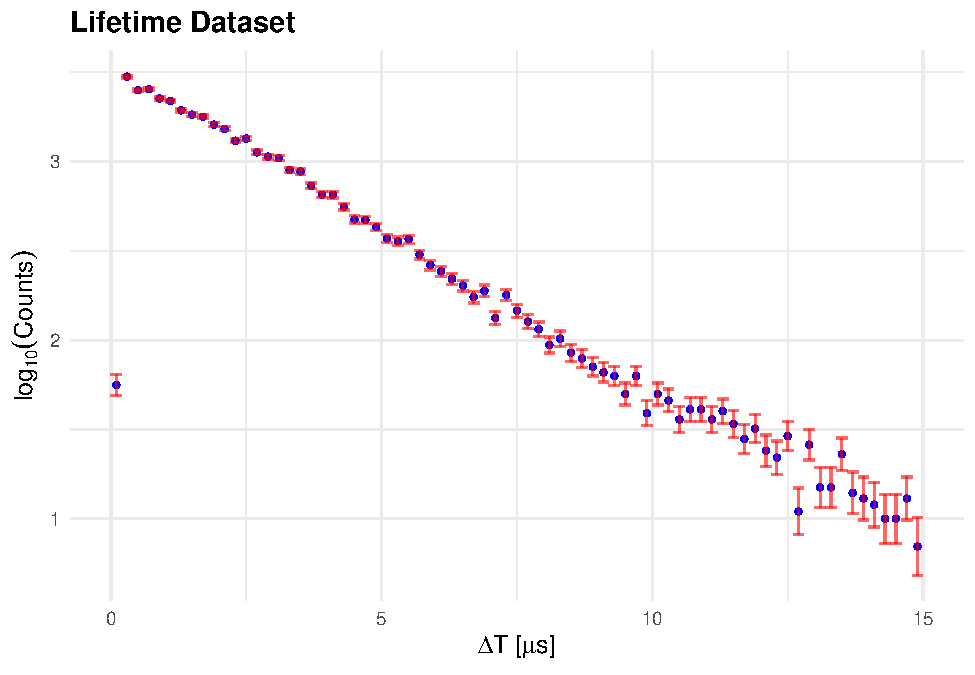
\includegraphics{BinnedAnalysis_files/figure-latex/unnamed-chunk-3-1.pdf}

\begin{Shaded}
\begin{Highlighting}[]
\FunctionTok{plotdata}\NormalTok{(data\_precession, }\AttributeTok{title =} \StringTok{\textquotesingle{}Precession Dataset\textquotesingle{}}\NormalTok{, }\AttributeTok{scale=}  \StringTok{\textquotesingle{}log\textquotesingle{}}\NormalTok{, }\AttributeTok{plot\_histbar =} \ConstantTok{FALSE}\NormalTok{)}
\end{Highlighting}
\end{Shaded}

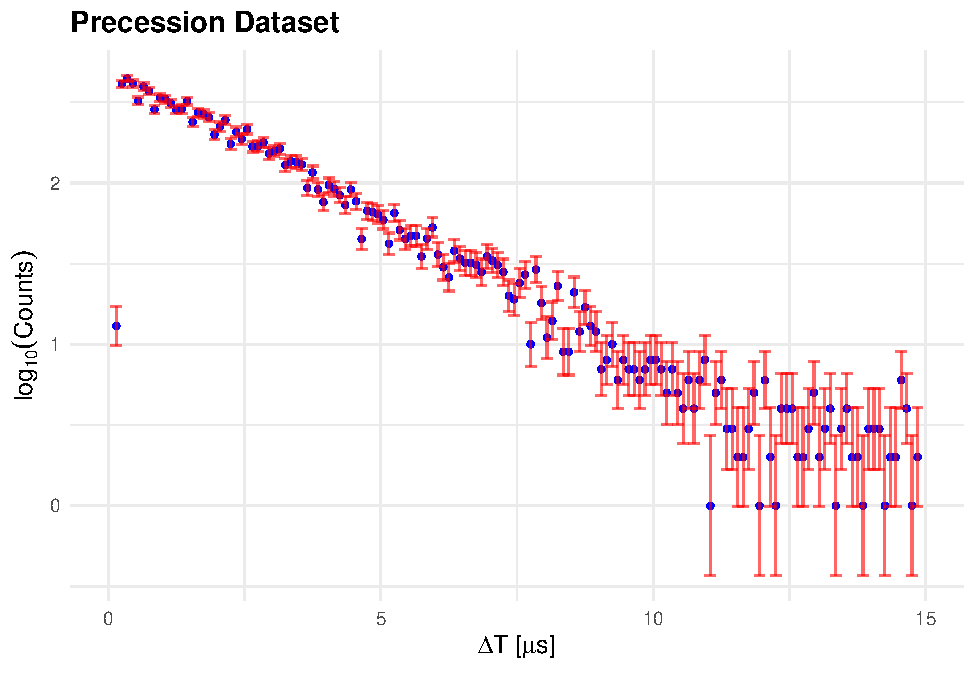
\includegraphics{BinnedAnalysis_files/figure-latex/unnamed-chunk-3-2.pdf}

\begin{Shaded}
\begin{Highlighting}[]
\NormalTok{lifetime\_hist}\OtherTok{\textless{}{-}}\FunctionTok{hist}\NormalTok{(data\_lifetime, }\AttributeTok{breaks=}\NormalTok{bins\_lifetime, }\AttributeTok{plot=}\ConstantTok{FALSE}\NormalTok{) }\CommentTok{\# from each dataset we create a df from a hist}
\NormalTok{filtered\_lifetime }\OtherTok{\textless{}{-}} \FunctionTok{data.frame}\NormalTok{(}\AttributeTok{mids =}\NormalTok{ lifetime\_hist}\SpecialCharTok{$}\NormalTok{mids, }\AttributeTok{counts =}\NormalTok{ lifetime\_hist}\SpecialCharTok{$}\NormalTok{counts)}
\NormalTok{filtered\_lifetime }\OtherTok{\textless{}{-}}\NormalTok{ filtered\_lifetime[}\SpecialCharTok{{-}}\DecValTok{1}\NormalTok{, ]}

\NormalTok{precession\_hist}\OtherTok{\textless{}{-}}\FunctionTok{hist}\NormalTok{(data\_precession, }\AttributeTok{breaks=}\NormalTok{bins\_default, }\AttributeTok{plot=}\ConstantTok{FALSE}\NormalTok{)}
\NormalTok{filtered\_precession }\OtherTok{\textless{}{-}} \FunctionTok{data.frame}\NormalTok{(}\AttributeTok{mids =}\NormalTok{ precession\_hist}\SpecialCharTok{$}\NormalTok{mids, }\AttributeTok{counts =}\NormalTok{ precession\_hist}\SpecialCharTok{$}\NormalTok{counts)}
\NormalTok{filtered\_precession }\OtherTok{\textless{}{-}}\NormalTok{ filtered\_precession[}\SpecialCharTok{{-}}\DecValTok{1}\NormalTok{, ]}

\FunctionTok{plotdata}\NormalTok{(data\_lifetime, }\AttributeTok{title =} \StringTok{\textquotesingle{}Lifetime\textquotesingle{}}\NormalTok{, }\AttributeTok{histdata =}\NormalTok{ filtered\_lifetime, }\AttributeTok{scale =} \StringTok{\textquotesingle{}log\textquotesingle{}}\NormalTok{, }\AttributeTok{plot\_histbar =} \ConstantTok{FALSE}\NormalTok{)}
\end{Highlighting}
\end{Shaded}

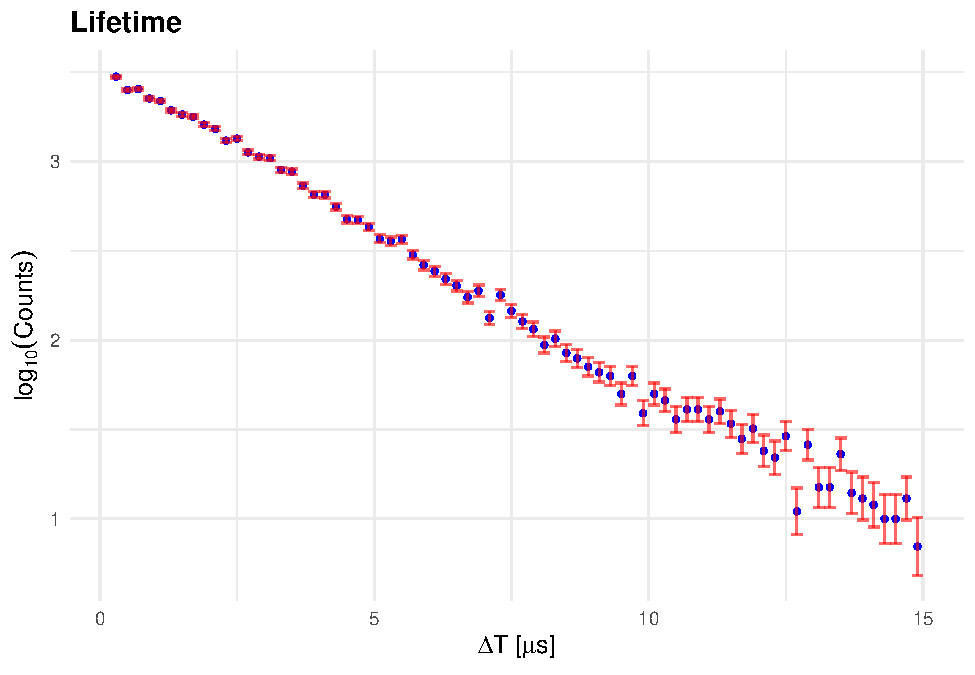
\includegraphics{BinnedAnalysis_files/figure-latex/unnamed-chunk-4-1.pdf}

\begin{Shaded}
\begin{Highlighting}[]
\FunctionTok{plotdata}\NormalTok{(data\_precession, }\AttributeTok{title =} \StringTok{\textquotesingle{}Precession\textquotesingle{}}\NormalTok{, }\AttributeTok{histdata =}\NormalTok{ filtered\_precession, }\AttributeTok{scale=}  \StringTok{\textquotesingle{}log\textquotesingle{}}\NormalTok{, }\AttributeTok{plot\_histbar =} \ConstantTok{FALSE}\NormalTok{)}
\end{Highlighting}
\end{Shaded}

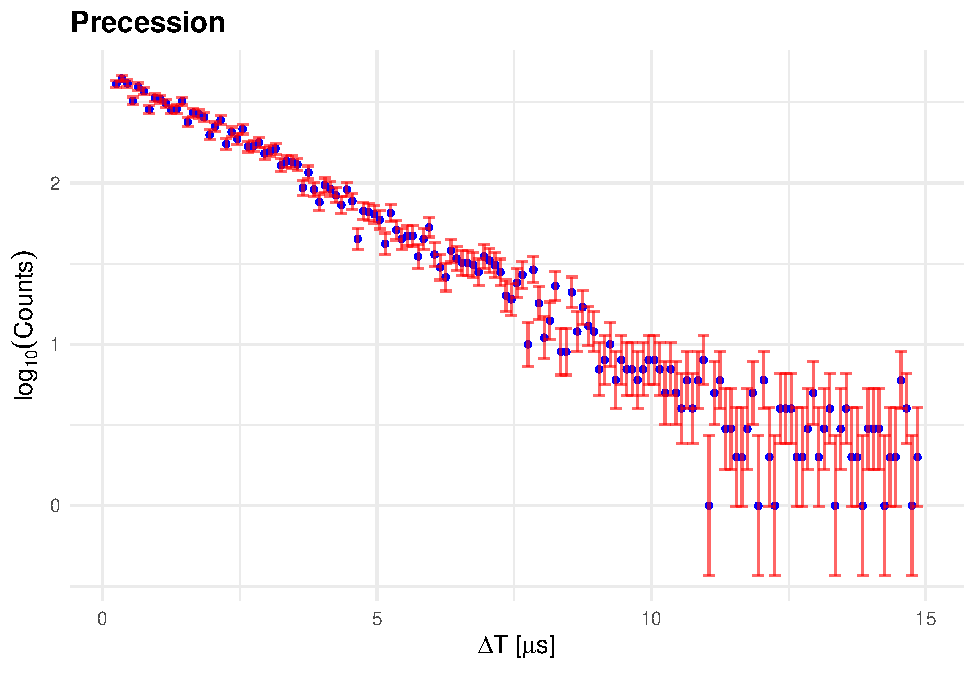
\includegraphics{BinnedAnalysis_files/figure-latex/unnamed-chunk-4-2.pdf}

\subsection{Lifetime analysis}\label{lifetime-analysis}

\begin{Shaded}
\begin{Highlighting}[]
\NormalTok{x }\OtherTok{\textless{}{-}}\NormalTok{ filtered\_lifetime}\SpecialCharTok{$}\NormalTok{mids}
\NormalTok{y }\OtherTok{\textless{}{-}}\NormalTok{ filtered\_lifetime}\SpecialCharTok{$}\NormalTok{counts}

\CommentTok{\# Define initial values for the chains}
\NormalTok{init\_values }\OtherTok{\textless{}{-}} \FunctionTok{list}\NormalTok{(}\FunctionTok{list}\NormalTok{(}\AttributeTok{N =} \DecValTok{10000}\NormalTok{, }\AttributeTok{c =} \DecValTok{5}\NormalTok{, }\AttributeTok{tau =} \FloatTok{2.}\NormalTok{))}

\NormalTok{n\_burnin }\OtherTok{\textless{}{-}} \DecValTok{5000}  \CommentTok{\# Length of the burn{-}in phase}
\NormalTok{thinning }\OtherTok{\textless{}{-}} \DecValTok{2}
\NormalTok{Nrep     }\OtherTok{\textless{}{-}} \FloatTok{1e5} \CommentTok{\# Number of values to simulate}
\NormalTok{n\_adapt  }\OtherTok{\textless{}{-}} \DecValTok{2000}


\CommentTok{\# Define the model string using sprintf}
\NormalTok{model\_lifetime\_def }\OtherTok{\textless{}{-}} \FunctionTok{sprintf}\NormalTok{(}\StringTok{"}
\StringTok{model\{}
\StringTok{  \# Likelihood}
\StringTok{  for (i in 1:length(x)) \{}
\StringTok{    I[i] \textless{}{-} N*exp({-}x[i]/tau) + c}
\StringTok{    y[i] \textasciitilde{} dpois(I[i])}
\StringTok{  \}}

\StringTok{  \# Prior}
\StringTok{  N \textasciitilde{} dunif(0, 20000)}
\StringTok{  c \textasciitilde{} dunif(0, 50)}
\StringTok{  tau \textasciitilde{} dgamma(\%.2f, \%.2f)}
\StringTok{\}"}\NormalTok{, PriorParam}\SpecialCharTok{$}\NormalTok{tau[[}\StringTok{"alpha"}\NormalTok{]], PriorParam}\SpecialCharTok{$}\NormalTok{tau[[}\StringTok{"beta"}\NormalTok{]])}

\NormalTok{dataList }\OtherTok{=} \FunctionTok{list}\NormalTok{(}\AttributeTok{x =}\NormalTok{ x, }\AttributeTok{y =}\NormalTok{ y)}

\CommentTok{\# Create the model}
\NormalTok{model\_lifetime }\OtherTok{\textless{}{-}} \FunctionTok{jags.model}\NormalTok{(}\AttributeTok{file =} \FunctionTok{textConnection}\NormalTok{(model\_lifetime\_def), }\AttributeTok{data =}\NormalTok{ dataList, }\AttributeTok{inits =}\NormalTok{ init\_values, }\AttributeTok{n.chains =} \DecValTok{1}\NormalTok{)}
\end{Highlighting}
\end{Shaded}

\begin{verbatim}
## Compiling model graph
##    Resolving undeclared variables
##    Allocating nodes
## Graph information:
##    Observed stochastic nodes: 74
##    Unobserved stochastic nodes: 3
##    Total graph size: 526
## 
## Initializing model
\end{verbatim}

\begin{Shaded}
\begin{Highlighting}[]
\CommentTok{\# Adaptation phase}
\FunctionTok{adapt}\NormalTok{(model\_lifetime, n\_adapt)}
\end{Highlighting}
\end{Shaded}

\begin{verbatim}
## [1] TRUE
\end{verbatim}

\begin{Shaded}
\begin{Highlighting}[]
\CommentTok{\# Burn{-}in phase}
\FunctionTok{update}\NormalTok{(model\_lifetime, }\AttributeTok{n.iter =}\NormalTok{ n\_burnin)}

\CommentTok{\# Sample from the posterior}
\NormalTok{posterior\_lifetime }\OtherTok{\textless{}{-}} \FunctionTok{coda.samples}\NormalTok{(model\_lifetime, }\AttributeTok{variable.names =} \FunctionTok{c}\NormalTok{(}\StringTok{\textquotesingle{}N\textquotesingle{}}\NormalTok{,}\StringTok{\textquotesingle{}c\textquotesingle{}}\NormalTok{,}\StringTok{\textquotesingle{}tau\textquotesingle{}}\NormalTok{), }\AttributeTok{n.iter =}\NormalTok{ Nrep, }\AttributeTok{thin =}\NormalTok{ thinning)}
\NormalTok{(summary\_lifetime }\OtherTok{\textless{}{-}} \FunctionTok{summary}\NormalTok{(posterior\_lifetime))}
\end{Highlighting}
\end{Shaded}

\begin{verbatim}
## 
## Iterations = 6002:106000
## Thinning interval = 2 
## Number of chains = 1 
## Sample size per chain = 50000 
## 
## 1. Empirical mean and standard deviation for each variable,
##    plus standard error of the mean:
## 
##         Mean        SD  Naive SE Time-series SE
## N   3698.532 23.841999 1.066e-01      1.407e-01
## c     10.988  1.020684 4.565e-03      5.332e-03
## tau    2.177  0.008451 3.779e-05      5.416e-05
## 
## 2. Quantiles for each variable:
## 
##         2.5%      25%      50%      75%    97.5%
## N   3652.305 3682.422 3698.384 3714.558 3745.813
## c      9.012   10.287   10.980   11.675   13.001
## tau    2.160    2.171    2.177    2.182    2.193
\end{verbatim}

\begin{Shaded}
\begin{Highlighting}[]
\FunctionTok{plot}\NormalTok{(posterior\_lifetime)}
\end{Highlighting}
\end{Shaded}

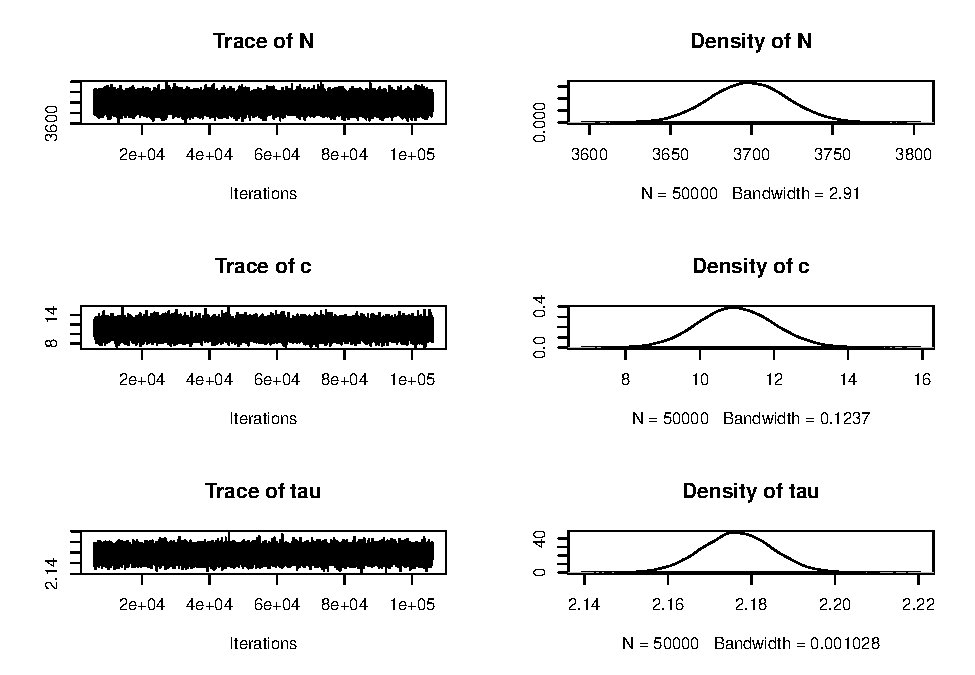
\includegraphics{BinnedAnalysis_files/figure-latex/unnamed-chunk-5-1.pdf}

\begin{Shaded}
\begin{Highlighting}[]
\NormalTok{posterior\_matrix }\OtherTok{\textless{}{-}} \FunctionTok{as.matrix}\NormalTok{(posterior\_lifetime)}

\CommentTok{\# Retrieve the chains}
\NormalTok{N\_samples   }\OtherTok{\textless{}{-}}\NormalTok{ posterior\_matrix[, }\StringTok{"N"}\NormalTok{]}
\NormalTok{c\_samples   }\OtherTok{\textless{}{-}}\NormalTok{ posterior\_matrix[, }\StringTok{"c"}\NormalTok{]}
\NormalTok{tau\_samples }\OtherTok{\textless{}{-}}\NormalTok{ posterior\_matrix[, }\StringTok{"tau"}\NormalTok{]}

\FunctionTok{par}\NormalTok{(}\AttributeTok{mfrow =} \FunctionTok{c}\NormalTok{(}\DecValTok{3}\NormalTok{, }\DecValTok{2}\NormalTok{))}

\FunctionTok{acf}\NormalTok{(N\_samples,  }\AttributeTok{main =} \StringTok{"Autocorrelation of N"}\NormalTok{)}
\FunctionTok{acf}\NormalTok{(c\_samples,   }\AttributeTok{main =} \StringTok{"Autocorrelation of c"}\NormalTok{)}
\FunctionTok{acf}\NormalTok{(tau\_samples, }\AttributeTok{main =} \StringTok{"Autocorrelation of tau"}\NormalTok{)}
\end{Highlighting}
\end{Shaded}

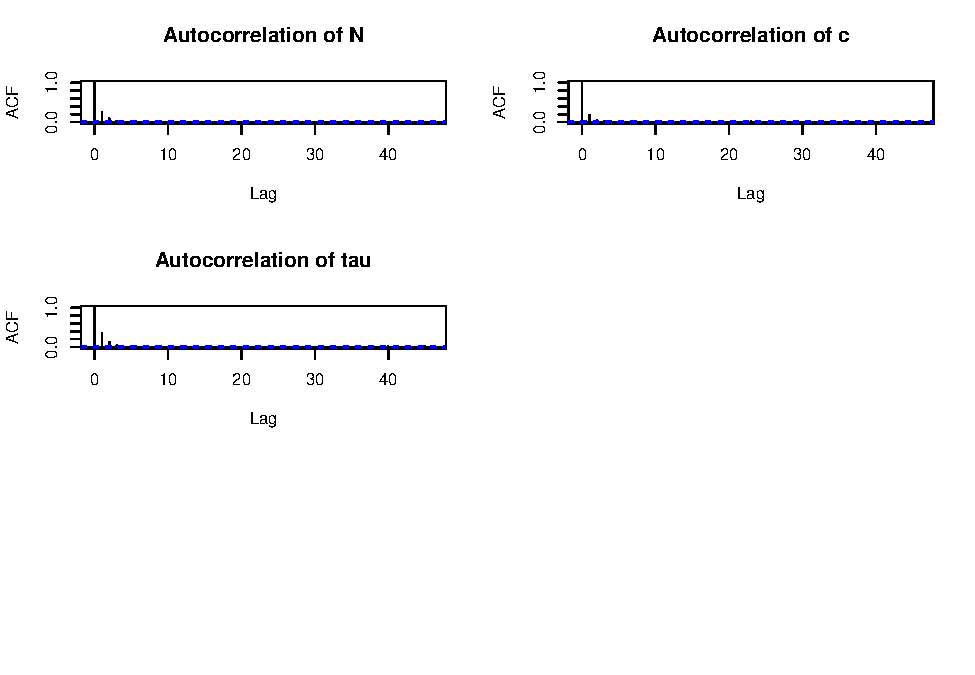
\includegraphics{BinnedAnalysis_files/figure-latex/unnamed-chunk-5-2.pdf}

\begin{Shaded}
\begin{Highlighting}[]
\NormalTok{N\_stats }\OtherTok{\textless{}{-}} \FunctionTok{extract\_stats}\NormalTok{(summary\_lifetime, }\StringTok{"N"}\NormalTok{)}
\NormalTok{c\_stats }\OtherTok{\textless{}{-}} \FunctionTok{extract\_stats}\NormalTok{(summary\_lifetime, }\StringTok{"c"}\NormalTok{)}
\NormalTok{tau\_stats }\OtherTok{\textless{}{-}} \FunctionTok{extract\_stats}\NormalTok{(summary\_lifetime, }\StringTok{"tau"}\NormalTok{)}

\NormalTok{prior\_tau }\OtherTok{\textless{}{-}} \ControlFlowTok{function}\NormalTok{(x) \{}
  \FunctionTok{dgamma}\NormalTok{(x, }\AttributeTok{shape =}\NormalTok{ PriorParam}\SpecialCharTok{$}\NormalTok{tau[[}\StringTok{"alpha"}\NormalTok{]], }\AttributeTok{rate =}\NormalTok{ PriorParam}\SpecialCharTok{$}\NormalTok{tau[[}\StringTok{"beta"}\NormalTok{]])}
\NormalTok{\}}

\FunctionTok{plot\_posterior\_param}\NormalTok{(N\_samples, }\StringTok{"N"}\NormalTok{, N\_stats)}
\end{Highlighting}
\end{Shaded}

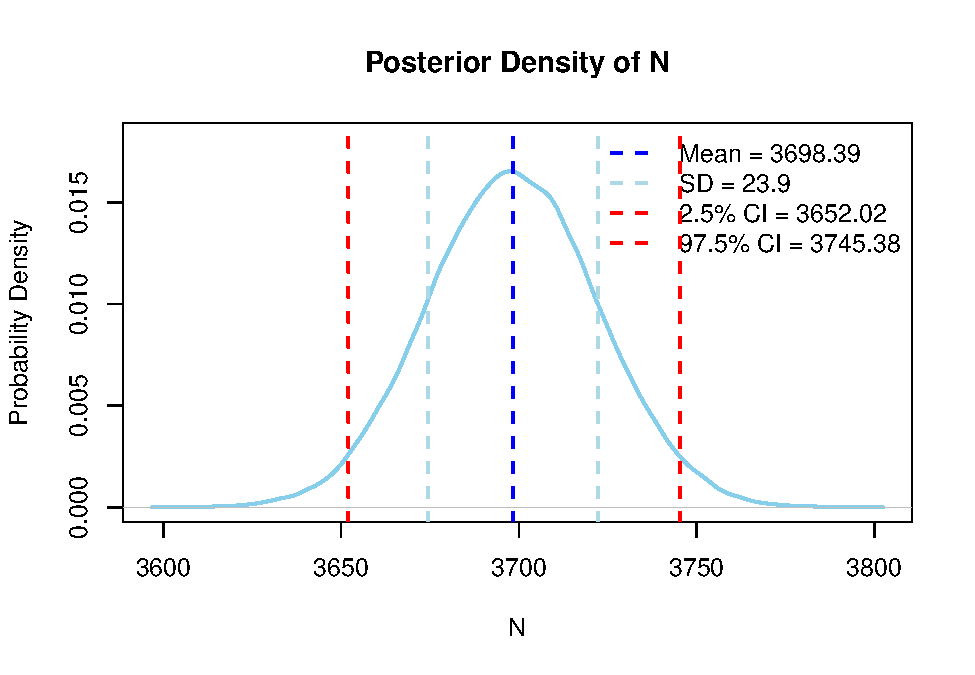
\includegraphics{BinnedAnalysis_files/figure-latex/unnamed-chunk-6-1.pdf}

\begin{Shaded}
\begin{Highlighting}[]
\FunctionTok{plot\_posterior\_param}\NormalTok{(c\_samples, }\StringTok{"c"}\NormalTok{, c\_stats)}
\end{Highlighting}
\end{Shaded}

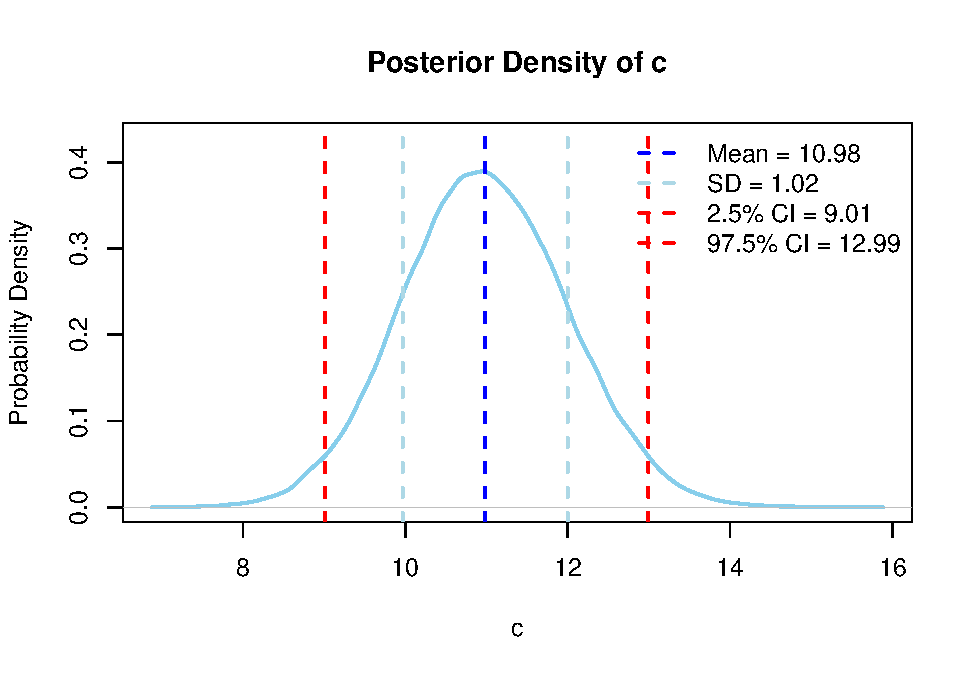
\includegraphics{BinnedAnalysis_files/figure-latex/unnamed-chunk-6-2.pdf}

\begin{Shaded}
\begin{Highlighting}[]
\FunctionTok{plot\_posterior\_param}\NormalTok{(tau\_samples, }\StringTok{"tau"}\NormalTok{, tau\_stats, prior\_tau, }\AttributeTok{xlim=}\FunctionTok{c}\NormalTok{(}\FloatTok{2.03}\NormalTok{,}\FloatTok{2.23}\NormalTok{), }\AttributeTok{xlab=}\FunctionTok{expression}\NormalTok{(tau }\SpecialCharTok{\textasciitilde{}} \StringTok{"["} \SpecialCharTok{*}\NormalTok{ mu }\SpecialCharTok{*} \StringTok{"s"} \SpecialCharTok{*} \StringTok{"]"}\NormalTok{), }\AttributeTok{legend.loc=}\StringTok{"topleft"}\NormalTok{)}
\end{Highlighting}
\end{Shaded}

\begin{verbatim}
## Warning in is.na(prior_func): is.na() applied to non-(list or vector) of type
## 'closure'
## Warning in is.na(prior_func): is.na() applied to non-(list or vector) of type
## 'closure'
\end{verbatim}

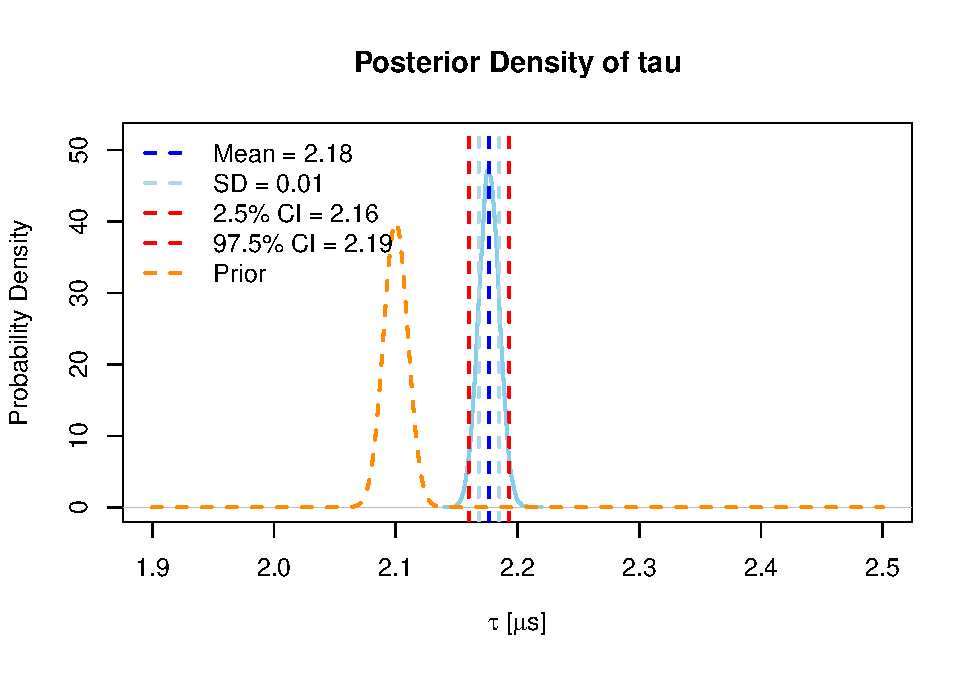
\includegraphics{BinnedAnalysis_files/figure-latex/unnamed-chunk-6-3.pdf}

\begin{Shaded}
\begin{Highlighting}[]
\FunctionTok{attributes}\NormalTok{(summary\_lifetime)}
\end{Highlighting}
\end{Shaded}

\begin{verbatim}
## $names
## [1] "statistics" "quantiles"  "start"      "end"        "thin"      
## [6] "nchain"    
## 
## $class
## [1] "summary.mcmc"
\end{verbatim}

\begin{Shaded}
\begin{Highlighting}[]
\NormalTok{parms\_lt }\OtherTok{\textless{}{-}}\NormalTok{ summary\_lifetime}\SpecialCharTok{$}\NormalTok{statistics[,}\StringTok{\textquotesingle{}Mean\textquotesingle{}}\NormalTok{]}

\NormalTok{lifetime\_law }\OtherTok{\textless{}{-}} \ControlFlowTok{function}\NormalTok{(x, parms) parms[}\StringTok{\textquotesingle{}N\textquotesingle{}}\NormalTok{] }\SpecialCharTok{*} \FunctionTok{exp}\NormalTok{(}\SpecialCharTok{{-}}\NormalTok{x}\SpecialCharTok{/}\NormalTok{parms[}\StringTok{\textquotesingle{}tau\textquotesingle{}}\NormalTok{]) }\SpecialCharTok{+}\NormalTok{ parms[}\StringTok{\textquotesingle{}c\textquotesingle{}}\NormalTok{]}

\FunctionTok{fitting}\NormalTok{(lifetime\_law,parms\_lt,data\_lifetime, }\AttributeTok{histdata =}\NormalTok{ filtered\_lifetime, }\AttributeTok{scale=}\StringTok{"lin"}\NormalTok{, }\AttributeTok{title=}\StringTok{\textquotesingle{}Fit of the Lifetime dataset\textquotesingle{}}\NormalTok{)}
\end{Highlighting}
\end{Shaded}

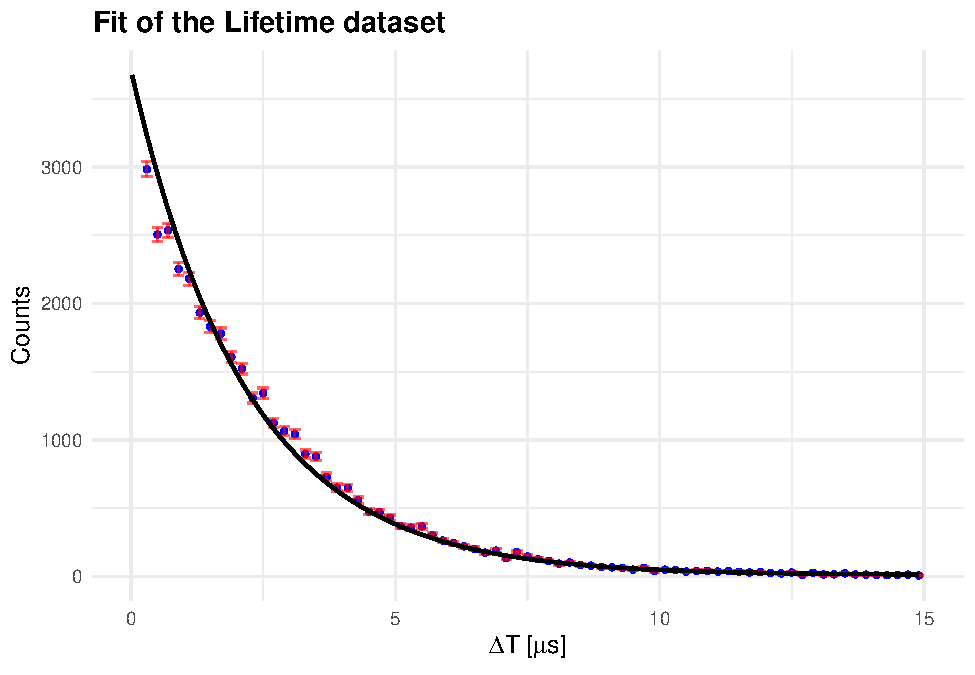
\includegraphics{BinnedAnalysis_files/figure-latex/unnamed-chunk-7-1.pdf}

\begin{Shaded}
\begin{Highlighting}[]
\FunctionTok{fitting}\NormalTok{(lifetime\_law,parms\_lt,data\_lifetime, }\AttributeTok{histdata =}\NormalTok{ filtered\_lifetime, }\AttributeTok{scale=}\StringTok{"log"}\NormalTok{, }\AttributeTok{title=}\StringTok{\textquotesingle{}Fit of the Lifetime dataset\textquotesingle{}}\NormalTok{)}
\end{Highlighting}
\end{Shaded}

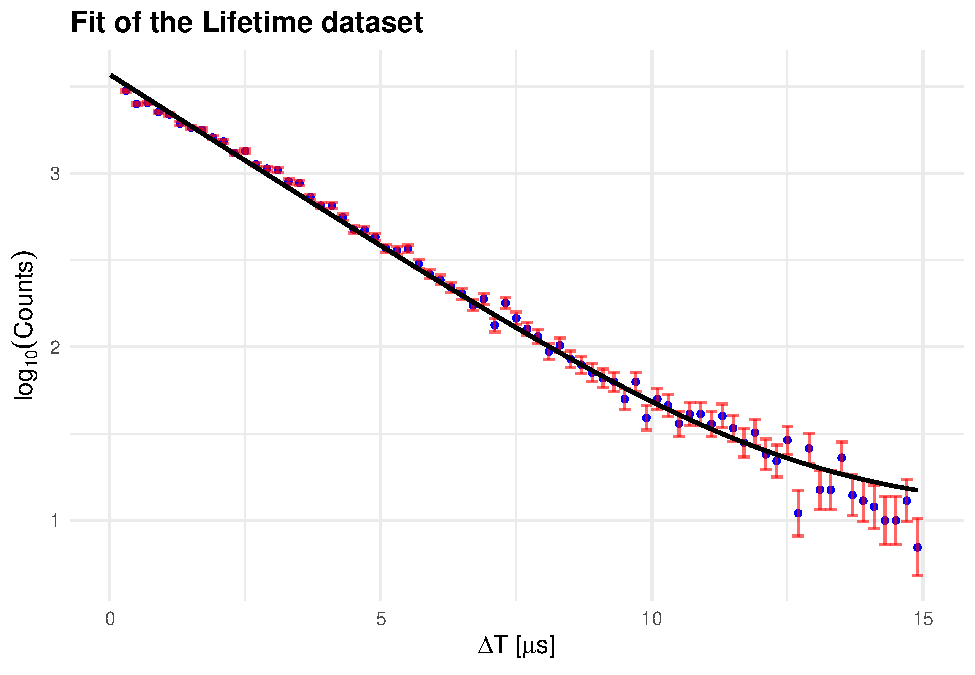
\includegraphics{BinnedAnalysis_files/figure-latex/unnamed-chunk-7-2.pdf}

\subsection{Precession Analysis}\label{precession-analysis}

\begin{Shaded}
\begin{Highlighting}[]
\NormalTok{tau\_lifetime\_posterior }\OtherTok{\textless{}{-}} \FunctionTok{getGammaParam}\NormalTok{(summary\_lifetime}\SpecialCharTok{$}\NormalTok{statistics[}\StringTok{\textquotesingle{}tau\textquotesingle{}}\NormalTok{, }\StringTok{\textquotesingle{}Mean\textquotesingle{}}\NormalTok{] ,summary\_lifetime}\SpecialCharTok{$}\NormalTok{statistics[}\StringTok{\textquotesingle{}tau\textquotesingle{}}\NormalTok{, }\StringTok{\textquotesingle{}SD\textquotesingle{}}\NormalTok{])}
\end{Highlighting}
\end{Shaded}

\begin{Shaded}
\begin{Highlighting}[]
\NormalTok{x }\OtherTok{\textless{}{-}}\NormalTok{ filtered\_precession}\SpecialCharTok{$}\NormalTok{mids}
\NormalTok{y }\OtherTok{\textless{}{-}}\NormalTok{ filtered\_precession}\SpecialCharTok{$}\NormalTok{counts}

\NormalTok{n\_burnin }\OtherTok{\textless{}{-}} \DecValTok{5000}  \CommentTok{\# Length of the burn{-}in phase}
\NormalTok{thinning }\OtherTok{\textless{}{-}} \DecValTok{2}
\NormalTok{Nrep     }\OtherTok{\textless{}{-}} \FloatTok{1e5} \CommentTok{\# Number of values to simulate}
\NormalTok{n\_adapt  }\OtherTok{\textless{}{-}} \DecValTok{1000}

\CommentTok{\# Define initial values for the chains}
\CommentTok{\#init\_values \textless{}{-} list(}
\CommentTok{\#  list(N = 500, c = 10, delta\_base = 0.4, omega = 4.7, alpha\_base = 0.05, tau=2.2)}
\CommentTok{\#)}

\NormalTok{init\_values }\OtherTok{\textless{}{-}} \FunctionTok{list}\NormalTok{(}
  \FunctionTok{list}\NormalTok{(}\AttributeTok{N =} \DecValTok{500}\NormalTok{, }\AttributeTok{c =} \DecValTok{10}\NormalTok{, }\AttributeTok{delta\_base =} \FloatTok{0.4}\NormalTok{, }\AttributeTok{omega =} \FloatTok{4.7}\NormalTok{, }\AttributeTok{alpha\_base =} \FloatTok{0.05}\NormalTok{)}
\NormalTok{)}

\CommentTok{\# Define the model string using sprintf}
\NormalTok{model\_precession\_def }\OtherTok{\textless{}{-}} \FunctionTok{sprintf}\NormalTok{(}\StringTok{"}
\StringTok{model\{}
\StringTok{  \# Likelihood}
\StringTok{  for (i in 1:length(x)) \{}
\StringTok{    I[i] \textless{}{-} N*exp({-}x[i]/tau) * (1 + alpha*cos(omega*x[i] + delta)) + c}
\StringTok{    y[i] \textasciitilde{} dpois(I[i])}
\StringTok{  \}}

\StringTok{  \# Prior}
\StringTok{  N \textasciitilde{} dunif(0, 15000)}
\StringTok{  c \textasciitilde{} dunif(0, 100)}

\StringTok{  delta\_base \textasciitilde{} dbeta(\%.2f, \%.2f)}
\StringTok{  omega \textasciitilde{} dgamma(\%.2f, \%.2f)}
\StringTok{  alpha\_base \textasciitilde{} dbeta(\%.2f, \%.2f)}
\StringTok{  \#tau \textasciitilde{} dgamma(\%.2f, \%.2f)}

\StringTok{  delta \textless{}{-} delta\_base * 3.14 {-} 3.14/2}
\StringTok{  alpha \textless{}{-} alpha\_base * 4/3 {-} 1/3}
\StringTok{  }
\StringTok{  g \textless{}{-} 0.41986*omega}
\StringTok{\}}
\StringTok{"}\NormalTok{, PriorParam}\SpecialCharTok{$}\NormalTok{delta[}\StringTok{"alpha"}\NormalTok{], PriorParam}\SpecialCharTok{$}\NormalTok{delta[}\StringTok{"beta"}\NormalTok{],}
\NormalTok{   PriorParam}\SpecialCharTok{$}\NormalTok{omega[}\StringTok{"alpha"}\NormalTok{], PriorParam}\SpecialCharTok{$}\NormalTok{omega[}\StringTok{"beta"}\NormalTok{],}
\NormalTok{   PriorParam}\SpecialCharTok{$}\NormalTok{alpha[}\StringTok{"alpha"}\NormalTok{], PriorParam}\SpecialCharTok{$}\NormalTok{alpha[}\StringTok{"beta"}\NormalTok{],}
\NormalTok{   tau\_lifetime\_posterior[}\StringTok{"alpha"}\NormalTok{], tau\_lifetime\_posterior[}\StringTok{"beta"}\NormalTok{])}

\NormalTok{dataList }\OtherTok{=} \FunctionTok{list}\NormalTok{(}\AttributeTok{x =}\NormalTok{ x, }\AttributeTok{y =}\NormalTok{ y, }\AttributeTok{tau=}\NormalTok{summary\_lifetime}\SpecialCharTok{$}\NormalTok{statistics[}\StringTok{\textquotesingle{}tau\textquotesingle{}}\NormalTok{, }\StringTok{\textquotesingle{}Mean\textquotesingle{}}\NormalTok{])}

\CommentTok{\# Create the model}
\NormalTok{model\_precession }\OtherTok{\textless{}{-}} \FunctionTok{jags.model}\NormalTok{(}\AttributeTok{file =} \FunctionTok{textConnection}\NormalTok{(model\_precession\_def), }\AttributeTok{data =}\NormalTok{ dataList, }\AttributeTok{inits =}\NormalTok{ init\_values, }\AttributeTok{n.chains =} \DecValTok{1}\NormalTok{)}
\end{Highlighting}
\end{Shaded}

\begin{verbatim}
## Compiling model graph
##    Resolving undeclared variables
##    Allocating nodes
## Graph information:
##    Observed stochastic nodes: 147
##    Unobserved stochastic nodes: 5
##    Total graph size: 1792
## 
## Initializing model
\end{verbatim}

\begin{Shaded}
\begin{Highlighting}[]
\CommentTok{\# Adaptation phase}
\FunctionTok{adapt}\NormalTok{(model\_precession, n\_adapt)}
\end{Highlighting}
\end{Shaded}

\begin{verbatim}
## [1] TRUE
\end{verbatim}

\begin{Shaded}
\begin{Highlighting}[]
\CommentTok{\# Burn{-}in phase}
\FunctionTok{update}\NormalTok{(model\_precession, }\AttributeTok{n.iter =}\NormalTok{ n\_burnin)}

\CommentTok{\# Sample from the posterior}
\NormalTok{posterior\_precession }\OtherTok{\textless{}{-}} \FunctionTok{coda.samples}\NormalTok{(model\_precession, }\AttributeTok{variable.names =} \FunctionTok{c}\NormalTok{(}\StringTok{\textquotesingle{}N\textquotesingle{}}\NormalTok{, }\StringTok{\textquotesingle{}c\textquotesingle{}}\NormalTok{, }\StringTok{\textquotesingle{}delta\textquotesingle{}}\NormalTok{, }\StringTok{\textquotesingle{}omega\textquotesingle{}}\NormalTok{, }\StringTok{\textquotesingle{}alpha\textquotesingle{}}\NormalTok{, }\StringTok{\textquotesingle{}g\textquotesingle{}}\NormalTok{, }\StringTok{\textquotesingle{}tau\textquotesingle{}}\NormalTok{), }\AttributeTok{n.iter =}\NormalTok{ Nrep, }\AttributeTok{thin =}\NormalTok{ thinning)}
\NormalTok{(summary\_precession }\OtherTok{\textless{}{-}} \FunctionTok{summary}\NormalTok{(posterior\_precession))}
\end{Highlighting}
\end{Shaded}

\begin{verbatim}
## 
## Iterations = 6002:106000
## Thinning interval = 2 
## Number of chains = 1 
## Sample size per chain = 50000 
## 
## 1. Empirical mean and standard deviation for each variable,
##    plus standard error of the mean:
## 
##            Mean      SD  Naive SE Time-series SE
## N     546.53981 5.59156 2.501e-02      2.784e-02
## alpha   0.03425 0.01136 5.079e-05      5.722e-05
## c       1.80361 0.26283 1.175e-03      1.313e-03
## delta  -0.04375 0.48575 2.172e-03      2.331e-03
## g       1.99150 0.02455 1.098e-04      1.189e-04
## omega   4.74324 0.05847 2.615e-04      2.833e-04
## tau     2.17653 0.00000 0.000e+00      0.000e+00
## 
## 2. Quantiles for each variable:
## 
##            2.5%       25%       50%       75%     97.5%
## N     535.59983 542.77637 546.55149 550.29650 557.45143
## alpha   0.01212   0.02655   0.03422   0.04186   0.05658
## c       1.30338   1.62384   1.79810   1.97786   2.33130
## delta  -1.00538  -0.36451  -0.05110   0.27068   0.94663
## g       1.94425   1.97461   1.99111   2.00795   2.04050
## omega   4.63071   4.70301   4.74231   4.78243   4.85996
## tau     2.17653   2.17653   2.17653   2.17653   2.17653
\end{verbatim}

\begin{Shaded}
\begin{Highlighting}[]
\NormalTok{posterior\_matrix }\OtherTok{\textless{}{-}} \FunctionTok{as.matrix}\NormalTok{(posterior\_precession)}

\CommentTok{\# Retrieve the chains}
\NormalTok{N\_samples    }\OtherTok{\textless{}{-}}\NormalTok{ posterior\_matrix[, }\StringTok{"N"}\NormalTok{]}
\NormalTok{c\_samples    }\OtherTok{\textless{}{-}}\NormalTok{ posterior\_matrix[, }\StringTok{"c"}\NormalTok{]}
\NormalTok{delta\_samples }\OtherTok{\textless{}{-}}\NormalTok{ posterior\_matrix[, }\StringTok{"delta"}\NormalTok{]}
\NormalTok{omega\_samples }\OtherTok{\textless{}{-}}\NormalTok{ posterior\_matrix[, }\StringTok{"omega"}\NormalTok{]}
\NormalTok{alpha\_samples }\OtherTok{\textless{}{-}}\NormalTok{ posterior\_matrix[, }\StringTok{"alpha"}\NormalTok{]}
\NormalTok{g\_samples }\OtherTok{\textless{}{-}}\NormalTok{ posterior\_matrix[, }\StringTok{"g"}\NormalTok{]}


\FunctionTok{acf}\NormalTok{(N\_samples, }\AttributeTok{main =} \StringTok{"Autocorrelation of N"}\NormalTok{)}
\end{Highlighting}
\end{Shaded}

\includegraphics{BinnedAnalysis_files/figure-latex/unnamed-chunk-9-1.pdf}

\begin{Shaded}
\begin{Highlighting}[]
\FunctionTok{acf}\NormalTok{(c\_samples, }\AttributeTok{main =} \StringTok{"Autocorrelation of c"}\NormalTok{)}
\end{Highlighting}
\end{Shaded}

\includegraphics{BinnedAnalysis_files/figure-latex/unnamed-chunk-9-2.pdf}

\begin{Shaded}
\begin{Highlighting}[]
\FunctionTok{acf}\NormalTok{(delta\_samples, }\AttributeTok{main =} \StringTok{"Autocorrelation of delta"}\NormalTok{)}
\end{Highlighting}
\end{Shaded}

\includegraphics{BinnedAnalysis_files/figure-latex/unnamed-chunk-9-3.pdf}

\begin{Shaded}
\begin{Highlighting}[]
\FunctionTok{acf}\NormalTok{(omega\_samples, }\AttributeTok{main =} \StringTok{"Autocorrelation of omega"}\NormalTok{)}
\end{Highlighting}
\end{Shaded}

\includegraphics{BinnedAnalysis_files/figure-latex/unnamed-chunk-9-4.pdf}

\begin{Shaded}
\begin{Highlighting}[]
\FunctionTok{acf}\NormalTok{(alpha\_samples, }\AttributeTok{main =} \StringTok{"Autocorrelation of alpha"}\NormalTok{)}
\end{Highlighting}
\end{Shaded}

\includegraphics{BinnedAnalysis_files/figure-latex/unnamed-chunk-9-5.pdf}

\begin{Shaded}
\begin{Highlighting}[]
\FunctionTok{acf}\NormalTok{(g\_samples, }\AttributeTok{main =} \StringTok{"Autocorrelation of g"}\NormalTok{)}
\end{Highlighting}
\end{Shaded}

\includegraphics{BinnedAnalysis_files/figure-latex/unnamed-chunk-9-6.pdf}

\begin{Shaded}
\begin{Highlighting}[]
\CommentTok{\# Extract statistics for each parameter}
\NormalTok{N\_stats }\OtherTok{\textless{}{-}} \FunctionTok{extract\_stats}\NormalTok{(summary\_precession, }\StringTok{"N"}\NormalTok{)}
\NormalTok{c\_stats }\OtherTok{\textless{}{-}} \FunctionTok{extract\_stats}\NormalTok{(summary\_precession, }\StringTok{"c"}\NormalTok{)}
\NormalTok{delta\_stats }\OtherTok{\textless{}{-}} \FunctionTok{extract\_stats}\NormalTok{(summary\_precession, }\StringTok{"delta"}\NormalTok{)}
\NormalTok{omega\_stats }\OtherTok{\textless{}{-}} \FunctionTok{extract\_stats}\NormalTok{(summary\_precession, }\StringTok{"omega"}\NormalTok{)}
\NormalTok{alpha\_stats }\OtherTok{\textless{}{-}} \FunctionTok{extract\_stats}\NormalTok{(summary\_precession, }\StringTok{"alpha"}\NormalTok{)}
\NormalTok{g\_stats }\OtherTok{\textless{}{-}} \FunctionTok{extract\_stats}\NormalTok{(summary\_precession, }\StringTok{"g"}\NormalTok{)}

\CommentTok{\# Define the prior functions for new parameters}
\NormalTok{prior\_delta }\OtherTok{\textless{}{-}} \ControlFlowTok{function}\NormalTok{(x) \{}
  \FunctionTok{dbeta}\NormalTok{((x }\SpecialCharTok{+} \FloatTok{3.14}\SpecialCharTok{/}\DecValTok{2}\NormalTok{) }\SpecialCharTok{/} \FloatTok{3.14}\NormalTok{, }\AttributeTok{shape1 =}\NormalTok{ PriorParam}\SpecialCharTok{$}\NormalTok{delta[}\StringTok{"alpha"}\NormalTok{], }\AttributeTok{shape2 =}\NormalTok{ PriorParam}\SpecialCharTok{$}\NormalTok{delta[}\StringTok{"beta"}\NormalTok{]) }\SpecialCharTok{/} \FloatTok{3.14}
\NormalTok{\}}

\NormalTok{prior\_omega }\OtherTok{\textless{}{-}} \ControlFlowTok{function}\NormalTok{(x) \{}
  \FunctionTok{dgamma}\NormalTok{(x, }\AttributeTok{shape =}\NormalTok{ PriorParam}\SpecialCharTok{$}\NormalTok{omega[}\StringTok{"alpha"}\NormalTok{], }\AttributeTok{rate =}\NormalTok{ PriorParam}\SpecialCharTok{$}\NormalTok{omega[}\StringTok{"beta"}\NormalTok{])}
\NormalTok{\}}

\NormalTok{prior\_alpha }\OtherTok{\textless{}{-}} \ControlFlowTok{function}\NormalTok{(x) \{}
  \FunctionTok{dbeta}\NormalTok{((x }\SpecialCharTok{+} \DecValTok{1}\SpecialCharTok{/}\DecValTok{3}\NormalTok{) }\SpecialCharTok{*} \DecValTok{3} \SpecialCharTok{/} \DecValTok{4}\NormalTok{, }\AttributeTok{shape1 =}\NormalTok{ PriorParam}\SpecialCharTok{$}\NormalTok{alpha[}\StringTok{"alpha"}\NormalTok{], }\AttributeTok{shape2 =}\NormalTok{ PriorParam}\SpecialCharTok{$}\NormalTok{alpha[}\StringTok{"beta"}\NormalTok{]) }\SpecialCharTok{*} \DecValTok{3} \SpecialCharTok{/} \DecValTok{4}
\NormalTok{\}}

\CommentTok{\# Plotting posterior parameters with priors}
\CommentTok{\#par(mfrow = c(5, 1))  \# Set up the plotting area for 5 plots vertically}

\FunctionTok{plot\_posterior\_param}\NormalTok{(N\_samples, }\StringTok{"N"}\NormalTok{, N\_stats)}
\end{Highlighting}
\end{Shaded}

\includegraphics{BinnedAnalysis_files/figure-latex/unnamed-chunk-10-1.pdf}

\begin{Shaded}
\begin{Highlighting}[]
\FunctionTok{plot\_posterior\_param}\NormalTok{(c\_samples, }\StringTok{"c"}\NormalTok{, c\_stats)}
\end{Highlighting}
\end{Shaded}

\includegraphics{BinnedAnalysis_files/figure-latex/unnamed-chunk-10-2.pdf}

\begin{Shaded}
\begin{Highlighting}[]
\FunctionTok{plot\_posterior\_param}\NormalTok{(delta\_samples, }\StringTok{"delta"}\NormalTok{, delta\_stats, prior\_delta, }\AttributeTok{xlab =} \FunctionTok{expression}\NormalTok{(delta }\SpecialCharTok{\textasciitilde{}} \StringTok{\textquotesingle{}[rad]\textquotesingle{}}\NormalTok{))}
\end{Highlighting}
\end{Shaded}

\begin{verbatim}
## Warning in is.na(prior_func): is.na() applied to non-(list or vector) of type
## 'closure'
## Warning in is.na(prior_func): is.na() applied to non-(list or vector) of type
## 'closure'
\end{verbatim}

\includegraphics{BinnedAnalysis_files/figure-latex/unnamed-chunk-10-3.pdf}

\begin{Shaded}
\begin{Highlighting}[]
\FunctionTok{plot\_posterior\_param}\NormalTok{(omega\_samples, }\StringTok{"omega"}\NormalTok{, omega\_stats, prior\_omega, }\AttributeTok{xlab =} \FunctionTok{expression}\NormalTok{(omega }\SpecialCharTok{\textasciitilde{}} \StringTok{\textquotesingle{}[MHz]\textquotesingle{}}\NormalTok{ ))}
\end{Highlighting}
\end{Shaded}

\begin{verbatim}
## Warning in is.na(prior_func): is.na() applied to non-(list or vector) of type
## 'closure'
## Warning in is.na(prior_func): is.na() applied to non-(list or vector) of type
## 'closure'
\end{verbatim}

\includegraphics{BinnedAnalysis_files/figure-latex/unnamed-chunk-10-4.pdf}

\begin{Shaded}
\begin{Highlighting}[]
\FunctionTok{plot\_posterior\_param}\NormalTok{(alpha\_samples, }\StringTok{"alpha"}\NormalTok{, alpha\_stats, prior\_alpha, }\AttributeTok{xlab =} \FunctionTok{expression}\NormalTok{(alpha), }\AttributeTok{xlim =} \FunctionTok{c}\NormalTok{(}\SpecialCharTok{{-}}\FloatTok{0.02}\NormalTok{, .}\DecValTok{12}\NormalTok{))}
\end{Highlighting}
\end{Shaded}

\begin{verbatim}
## Warning in is.na(prior_func): is.na() applied to non-(list or vector) of type
## 'closure'
## Warning in is.na(prior_func): is.na() applied to non-(list or vector) of type
## 'closure'
\end{verbatim}

\includegraphics{BinnedAnalysis_files/figure-latex/unnamed-chunk-10-5.pdf}

\begin{Shaded}
\begin{Highlighting}[]
\FunctionTok{plot\_posterior\_param}\NormalTok{(g\_samples, }\StringTok{"g"}\NormalTok{, g\_stats, }\AttributeTok{xlab=}\FunctionTok{expression}\NormalTok{(}\StringTok{\textquotesingle{}g\textquotesingle{}} \SpecialCharTok{*}\NormalTok{ mu))}
\end{Highlighting}
\end{Shaded}

\includegraphics{BinnedAnalysis_files/figure-latex/unnamed-chunk-10-6.pdf}

\begin{Shaded}
\begin{Highlighting}[]
\NormalTok{precession\_law }\OtherTok{\textless{}{-}} \ControlFlowTok{function}\NormalTok{(x, parms) \{}
\NormalTok{  parms[}\StringTok{\textquotesingle{}N\textquotesingle{}}\NormalTok{] }\SpecialCharTok{*} \FunctionTok{exp}\NormalTok{(}\SpecialCharTok{{-}}\NormalTok{x }\SpecialCharTok{/}\NormalTok{ parms[}\StringTok{\textquotesingle{}tau\textquotesingle{}}\NormalTok{]) }\SpecialCharTok{*}\NormalTok{ (}\DecValTok{1} \SpecialCharTok{+}\NormalTok{ parms[}\StringTok{\textquotesingle{}alpha\textquotesingle{}}\NormalTok{] }\SpecialCharTok{*} \FunctionTok{cos}\NormalTok{(parms[}\StringTok{\textquotesingle{}omega\textquotesingle{}}\NormalTok{] }\SpecialCharTok{*}\NormalTok{ x }\SpecialCharTok{+}\NormalTok{ parms[}\StringTok{\textquotesingle{}delta\textquotesingle{}}\NormalTok{])) }\SpecialCharTok{+}\NormalTok{ parms[}\StringTok{\textquotesingle{}c\textquotesingle{}}\NormalTok{]}
\NormalTok{\}}

\NormalTok{parms\_precession }\OtherTok{\textless{}{-}} \FunctionTok{summary}\NormalTok{(posterior\_precession)}\SpecialCharTok{$}\NormalTok{statistics[,}\StringTok{\textquotesingle{}Mean\textquotesingle{}}\NormalTok{]}

\FunctionTok{fitting}\NormalTok{(precession\_law, parms\_precession, data\_precession, }\AttributeTok{title=}\StringTok{\textquotesingle{}Precession\textquotesingle{}}\NormalTok{, }\AttributeTok{scale=}\StringTok{\textquotesingle{}lin\textquotesingle{}}\NormalTok{, }\AttributeTok{histdata=}\NormalTok{filtered\_precession)}
\end{Highlighting}
\end{Shaded}

\includegraphics{BinnedAnalysis_files/figure-latex/unnamed-chunk-11-1.pdf}

\begin{Shaded}
\begin{Highlighting}[]
\FunctionTok{fitting}\NormalTok{(precession\_law, parms\_precession, data\_precession, }\AttributeTok{title=}\StringTok{\textquotesingle{}Precession\textquotesingle{}}\NormalTok{, }\AttributeTok{scale=}\StringTok{\textquotesingle{}log\textquotesingle{}}\NormalTok{, }\AttributeTok{histdata=}\NormalTok{filtered\_precession)}
\end{Highlighting}
\end{Shaded}

\includegraphics{BinnedAnalysis_files/figure-latex/unnamed-chunk-11-2.pdf}

\end{document}
